\chapter{Model Activations}

The following figures show PCA representations of activations extracted from LLMs. Activations were obtained from three types of layers: Attention, MLP, and Hidden. Hallucinatory instances are indicated in red, while truthful ones are in blue.
\newpage
\begin{figure}[H]
    \centering
    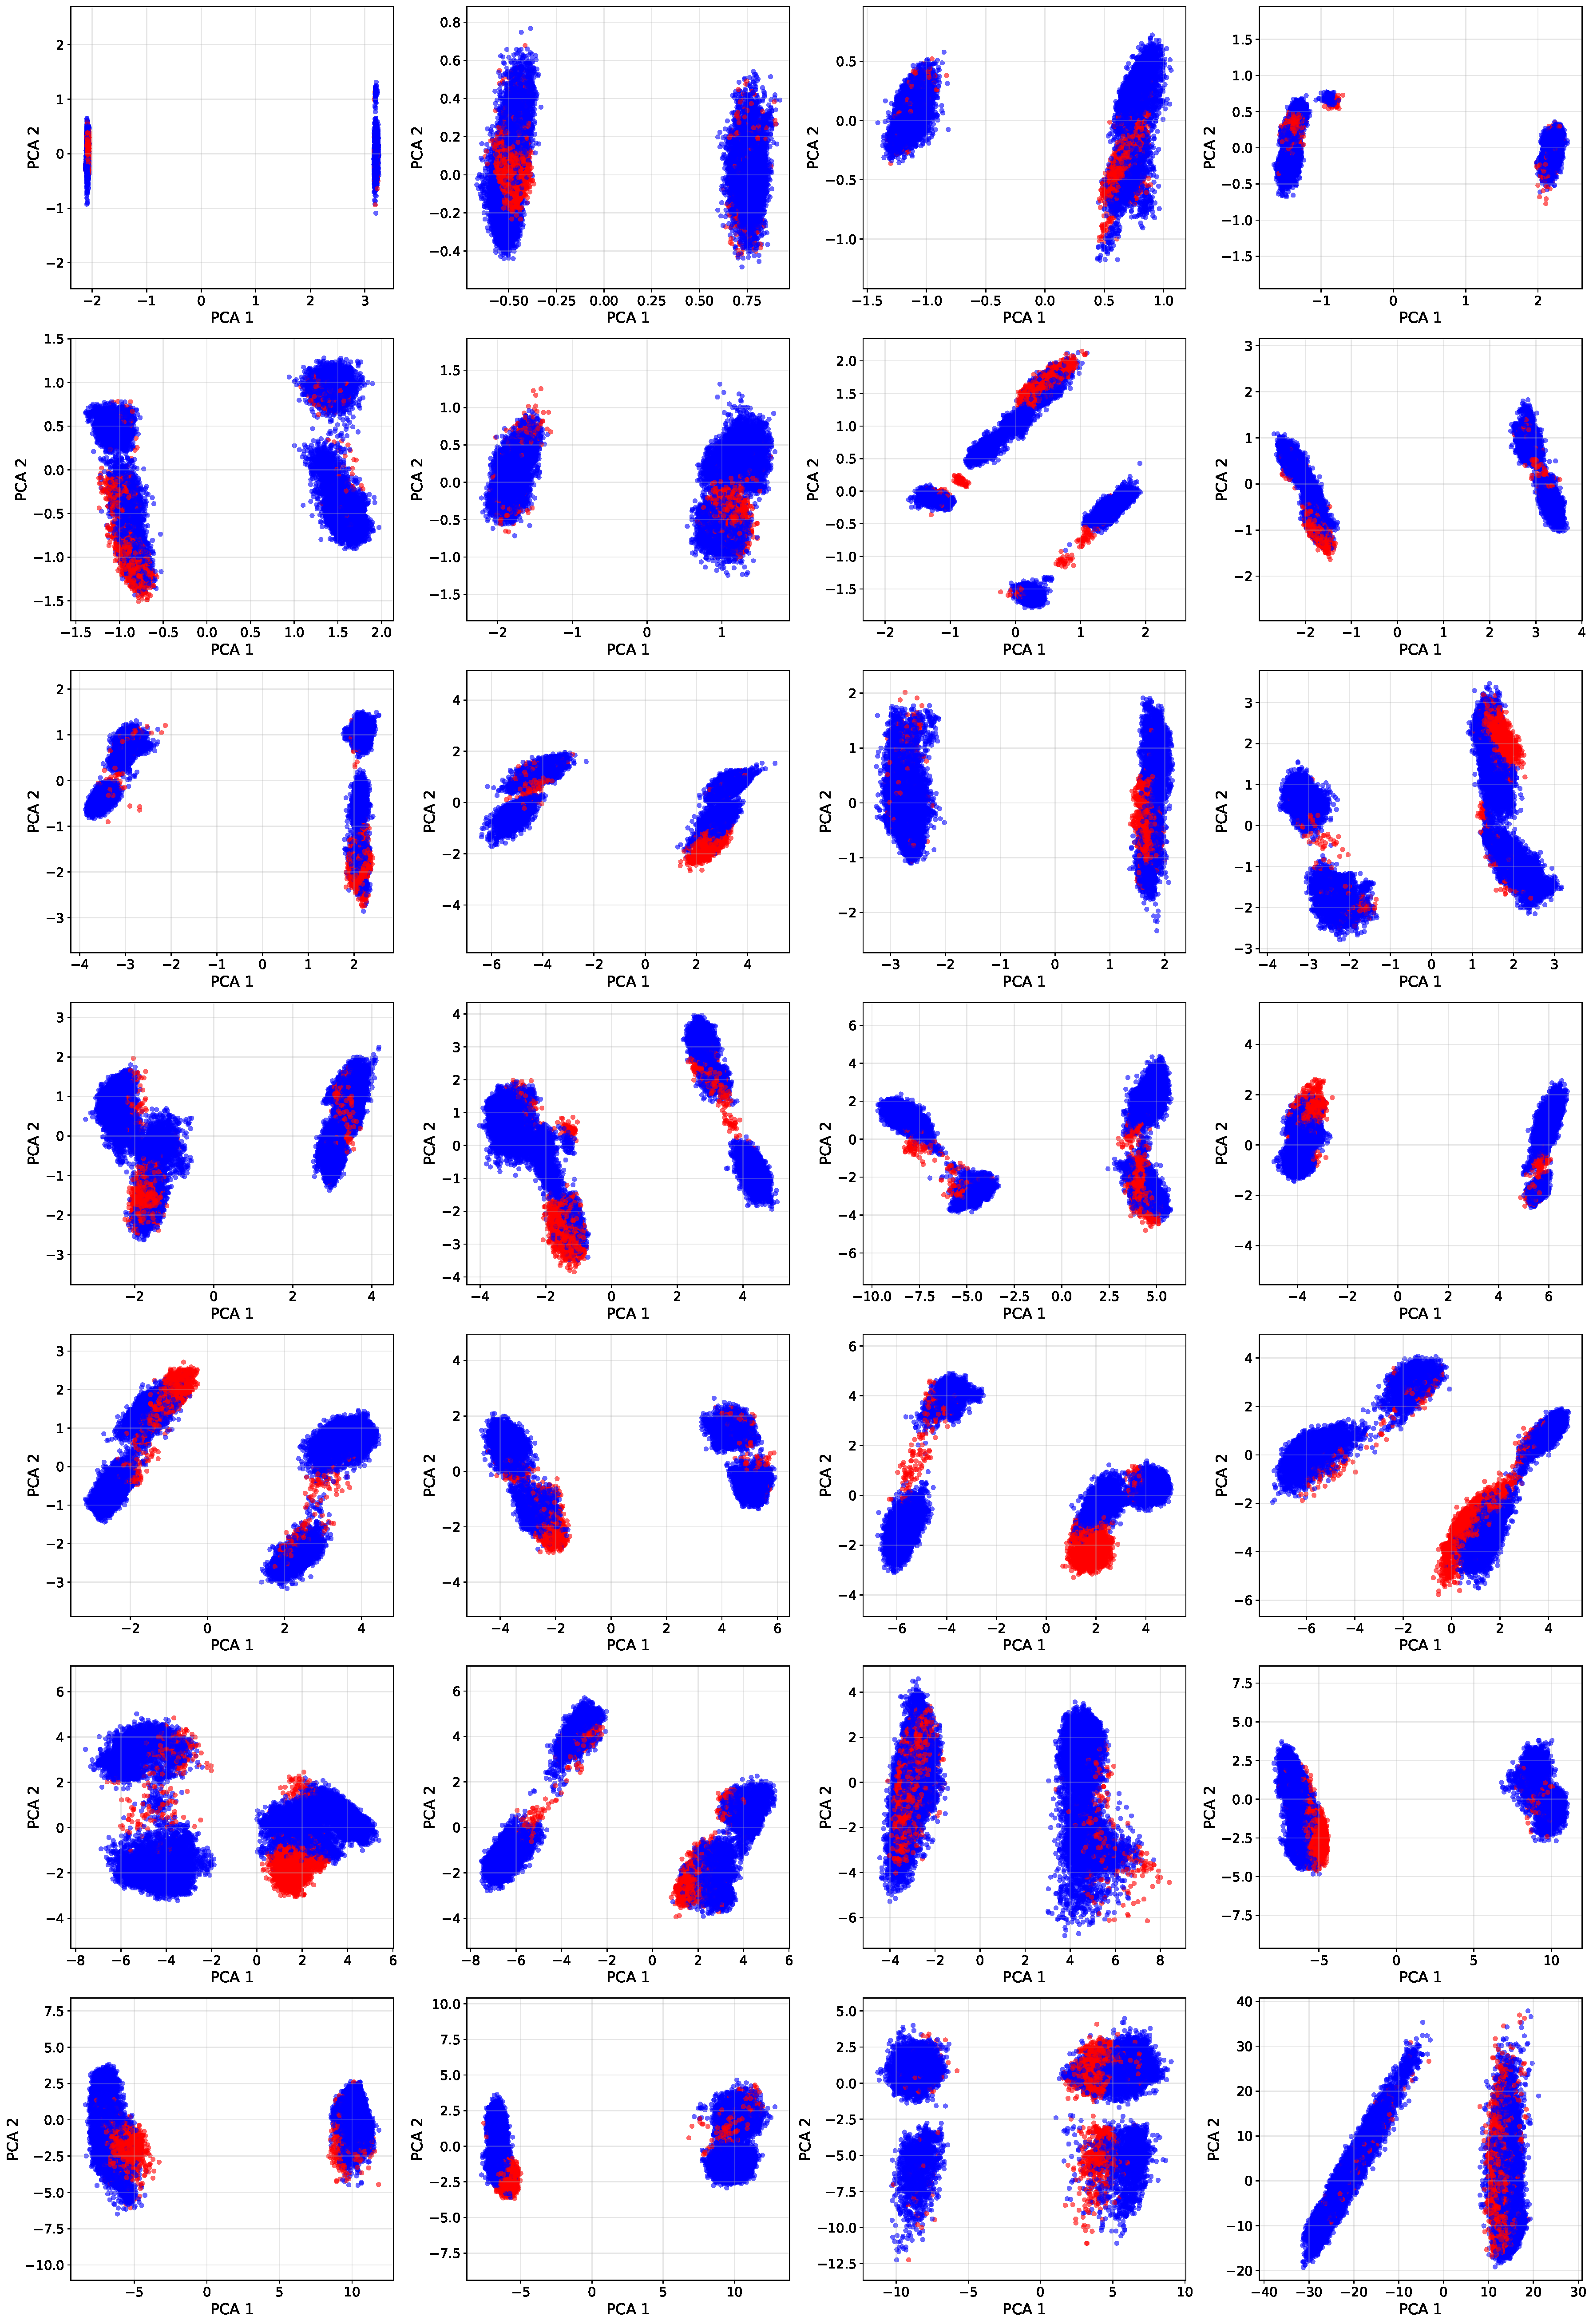
\includegraphics[width=\textwidth, height=1\textheight, keepaspectratio]{images/PCA_Plots/Qwen2.5-7B_belief_bank_facts_attn_activations_PCA_CLEAN.pdf}
    \caption{PCA of Attention layer activations from Qwen2.5-7B for Belief Bank Facts}
    \label{fig:qwen-pca-attn-facts-full}
\end{figure}

\begin{figure}[H]
    \centering
    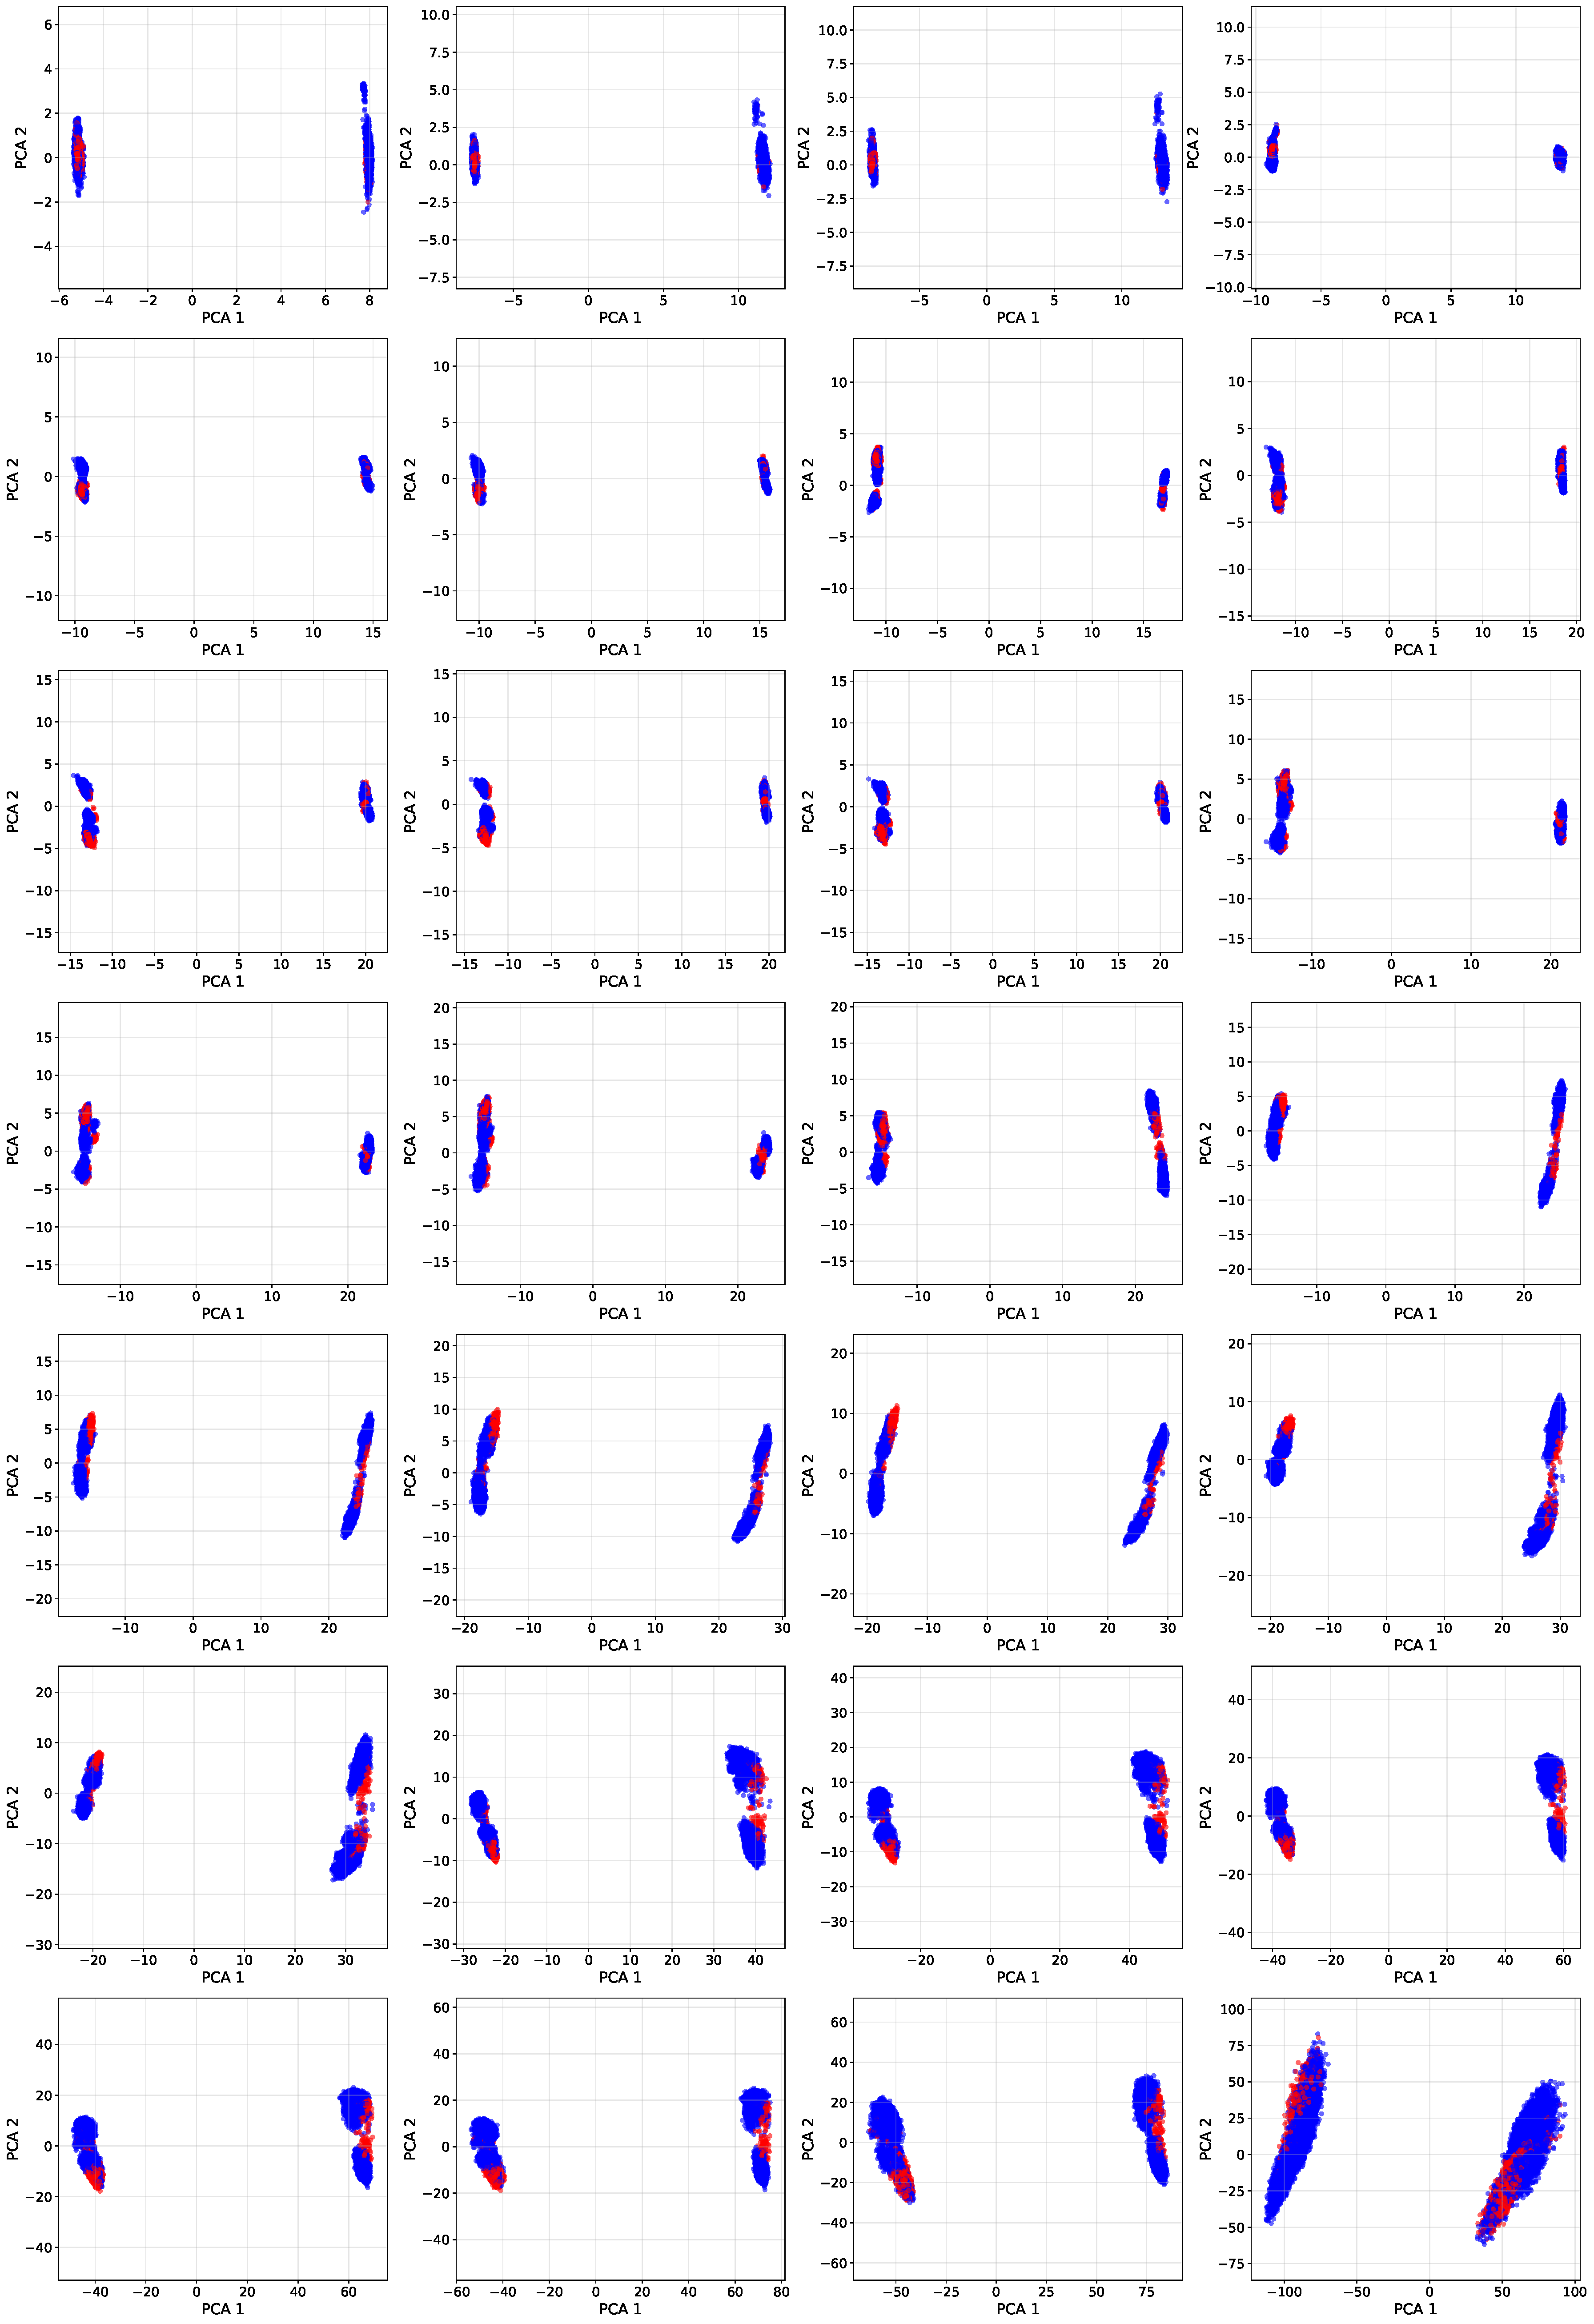
\includegraphics[width=\textwidth, height=1\textheight, keepaspectratio]{images/PCA_Plots/Qwen2.5-7B_belief_bank_facts_hidden_activations_PCA_CLEAN.pdf}
    \caption{PCA of Hidden layer activations from Qwen2.5-7B for Belief Bank Facts}

    \label{fig:qwen-pca-hidden-facts-full}
\end{figure}

\begin{figure}[H]
    \centering
    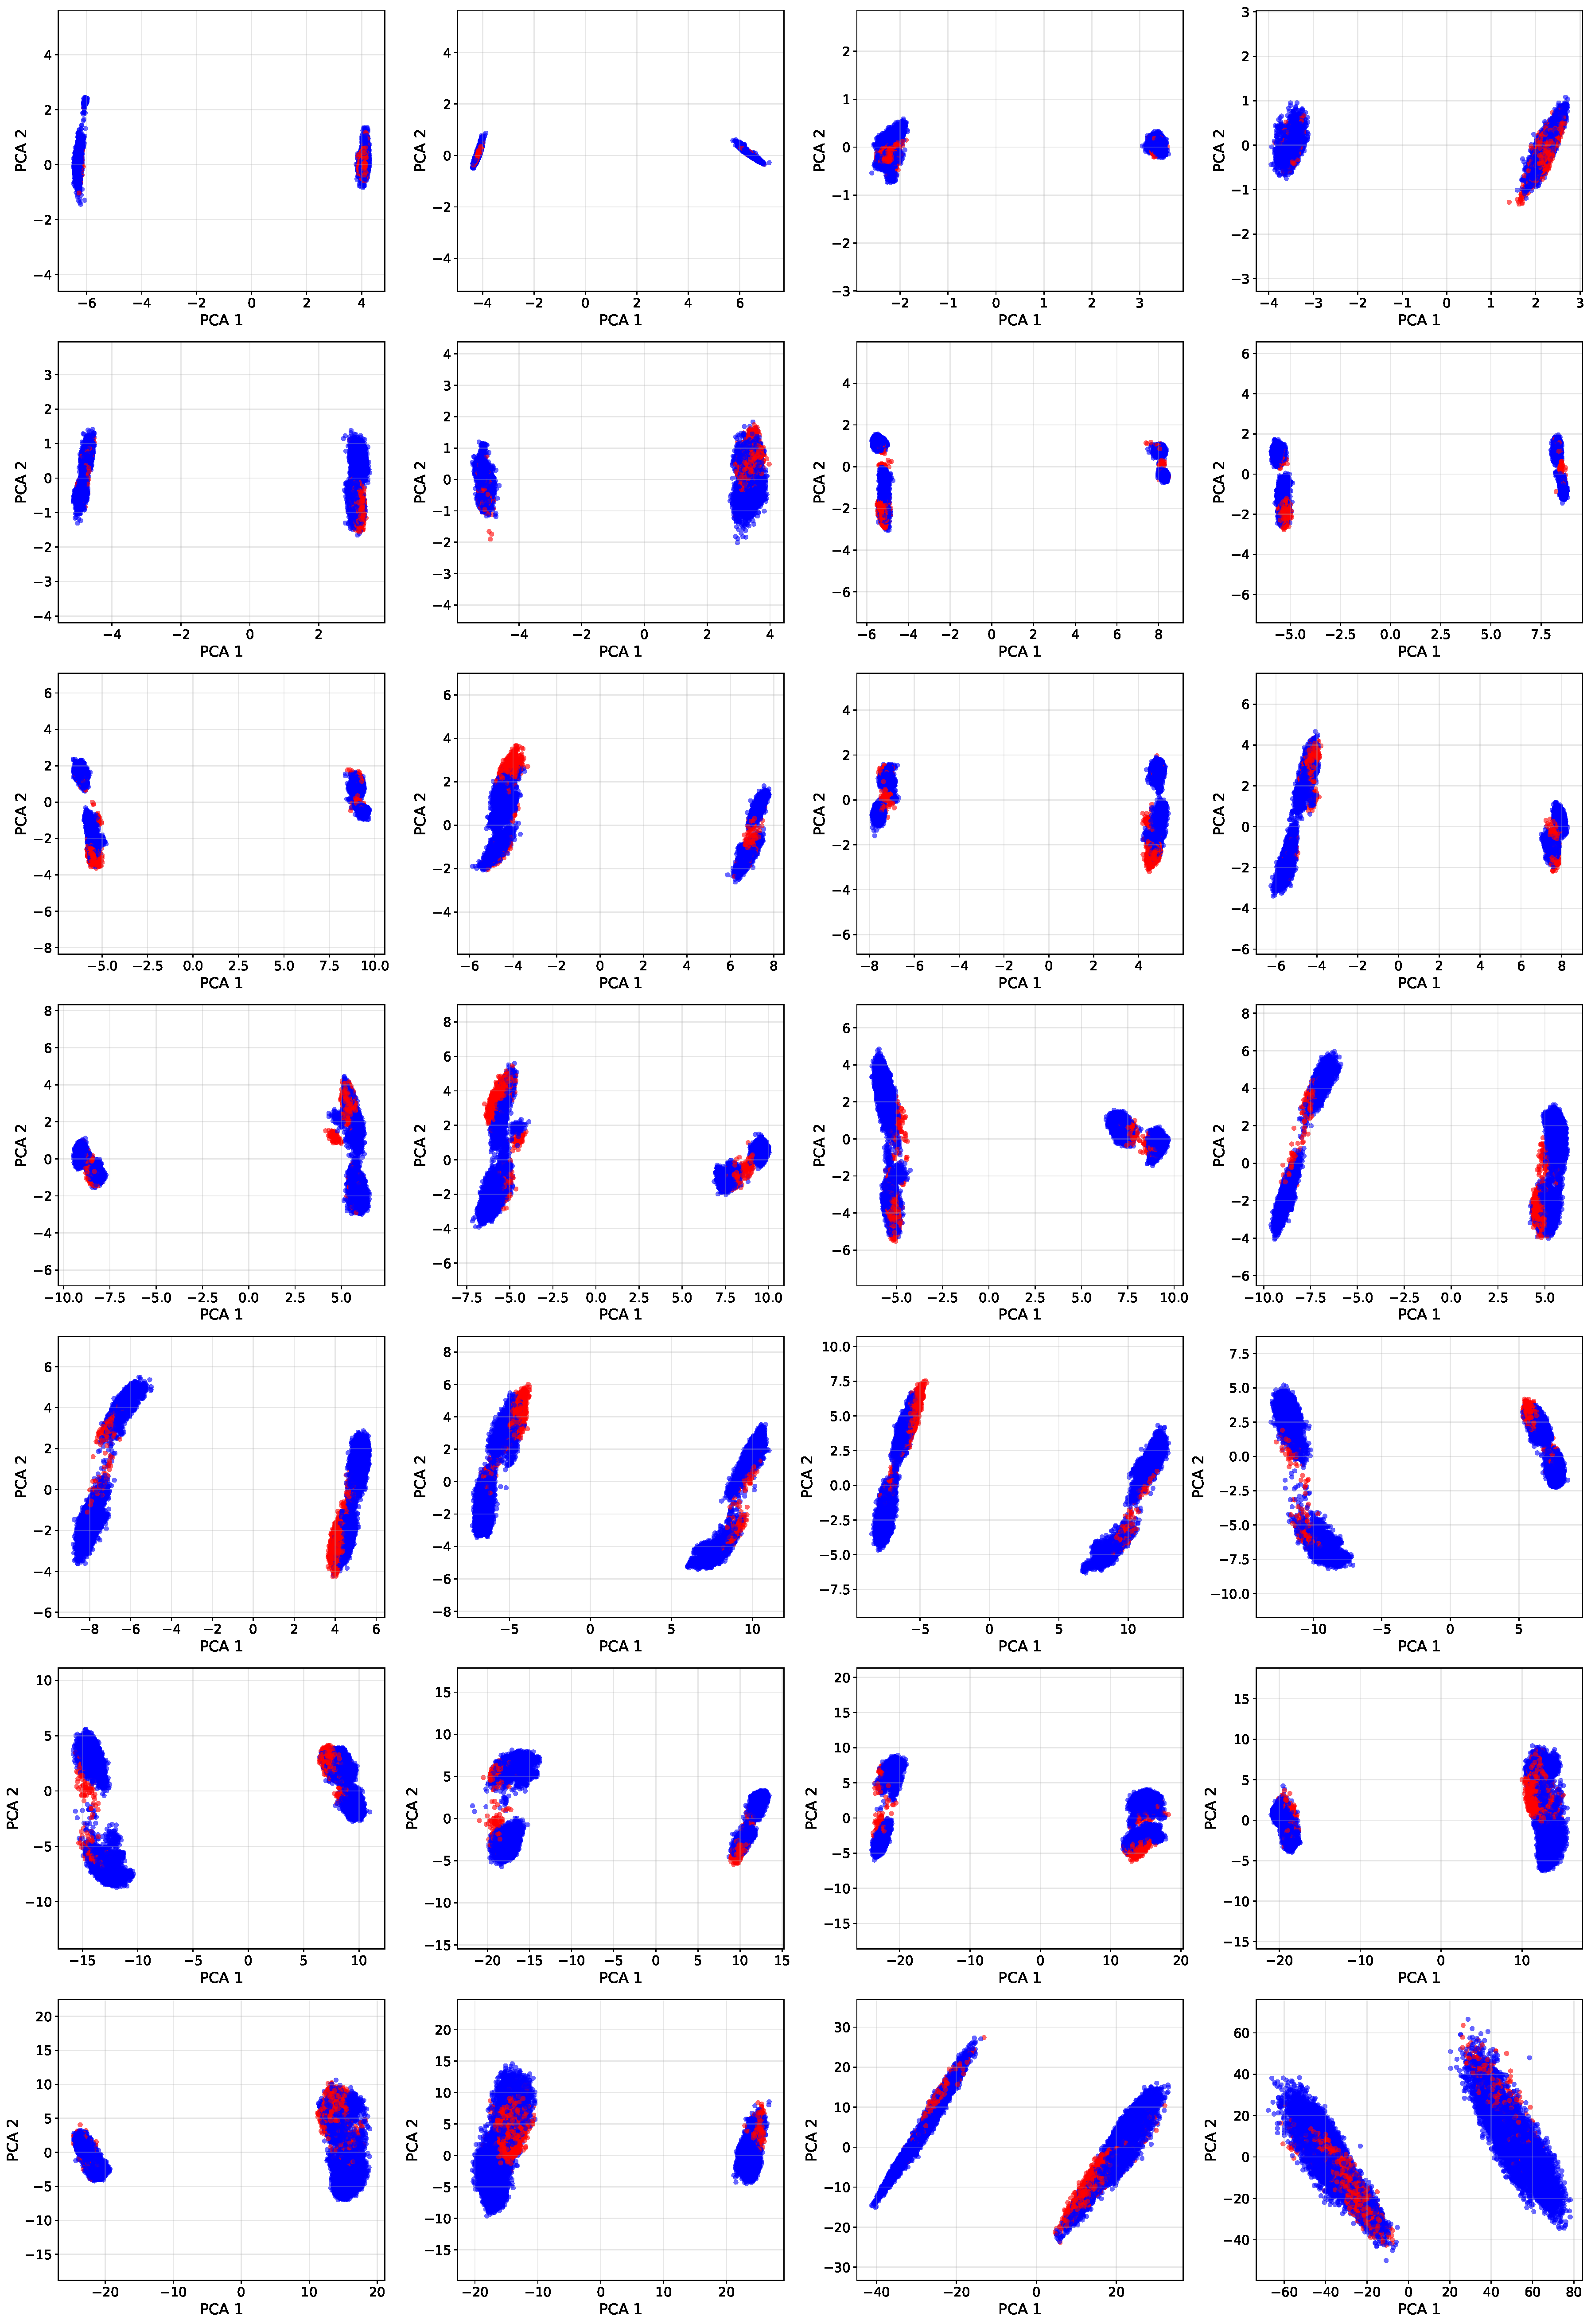
\includegraphics[width=\textwidth, height=1\textheight, keepaspectratio]{images/PCA_Plots/Qwen2.5-7B_belief_bank_facts_mlp_activations_PCA_CLEAN.pdf}
    \caption{PCA of MLP layer activations from Qwen2.5-7B for Belief Bank Facts}

    \label{fig:qwen-pca-mlp-facts-full}
\end{figure}


\begin{figure}[H]
    \centering
    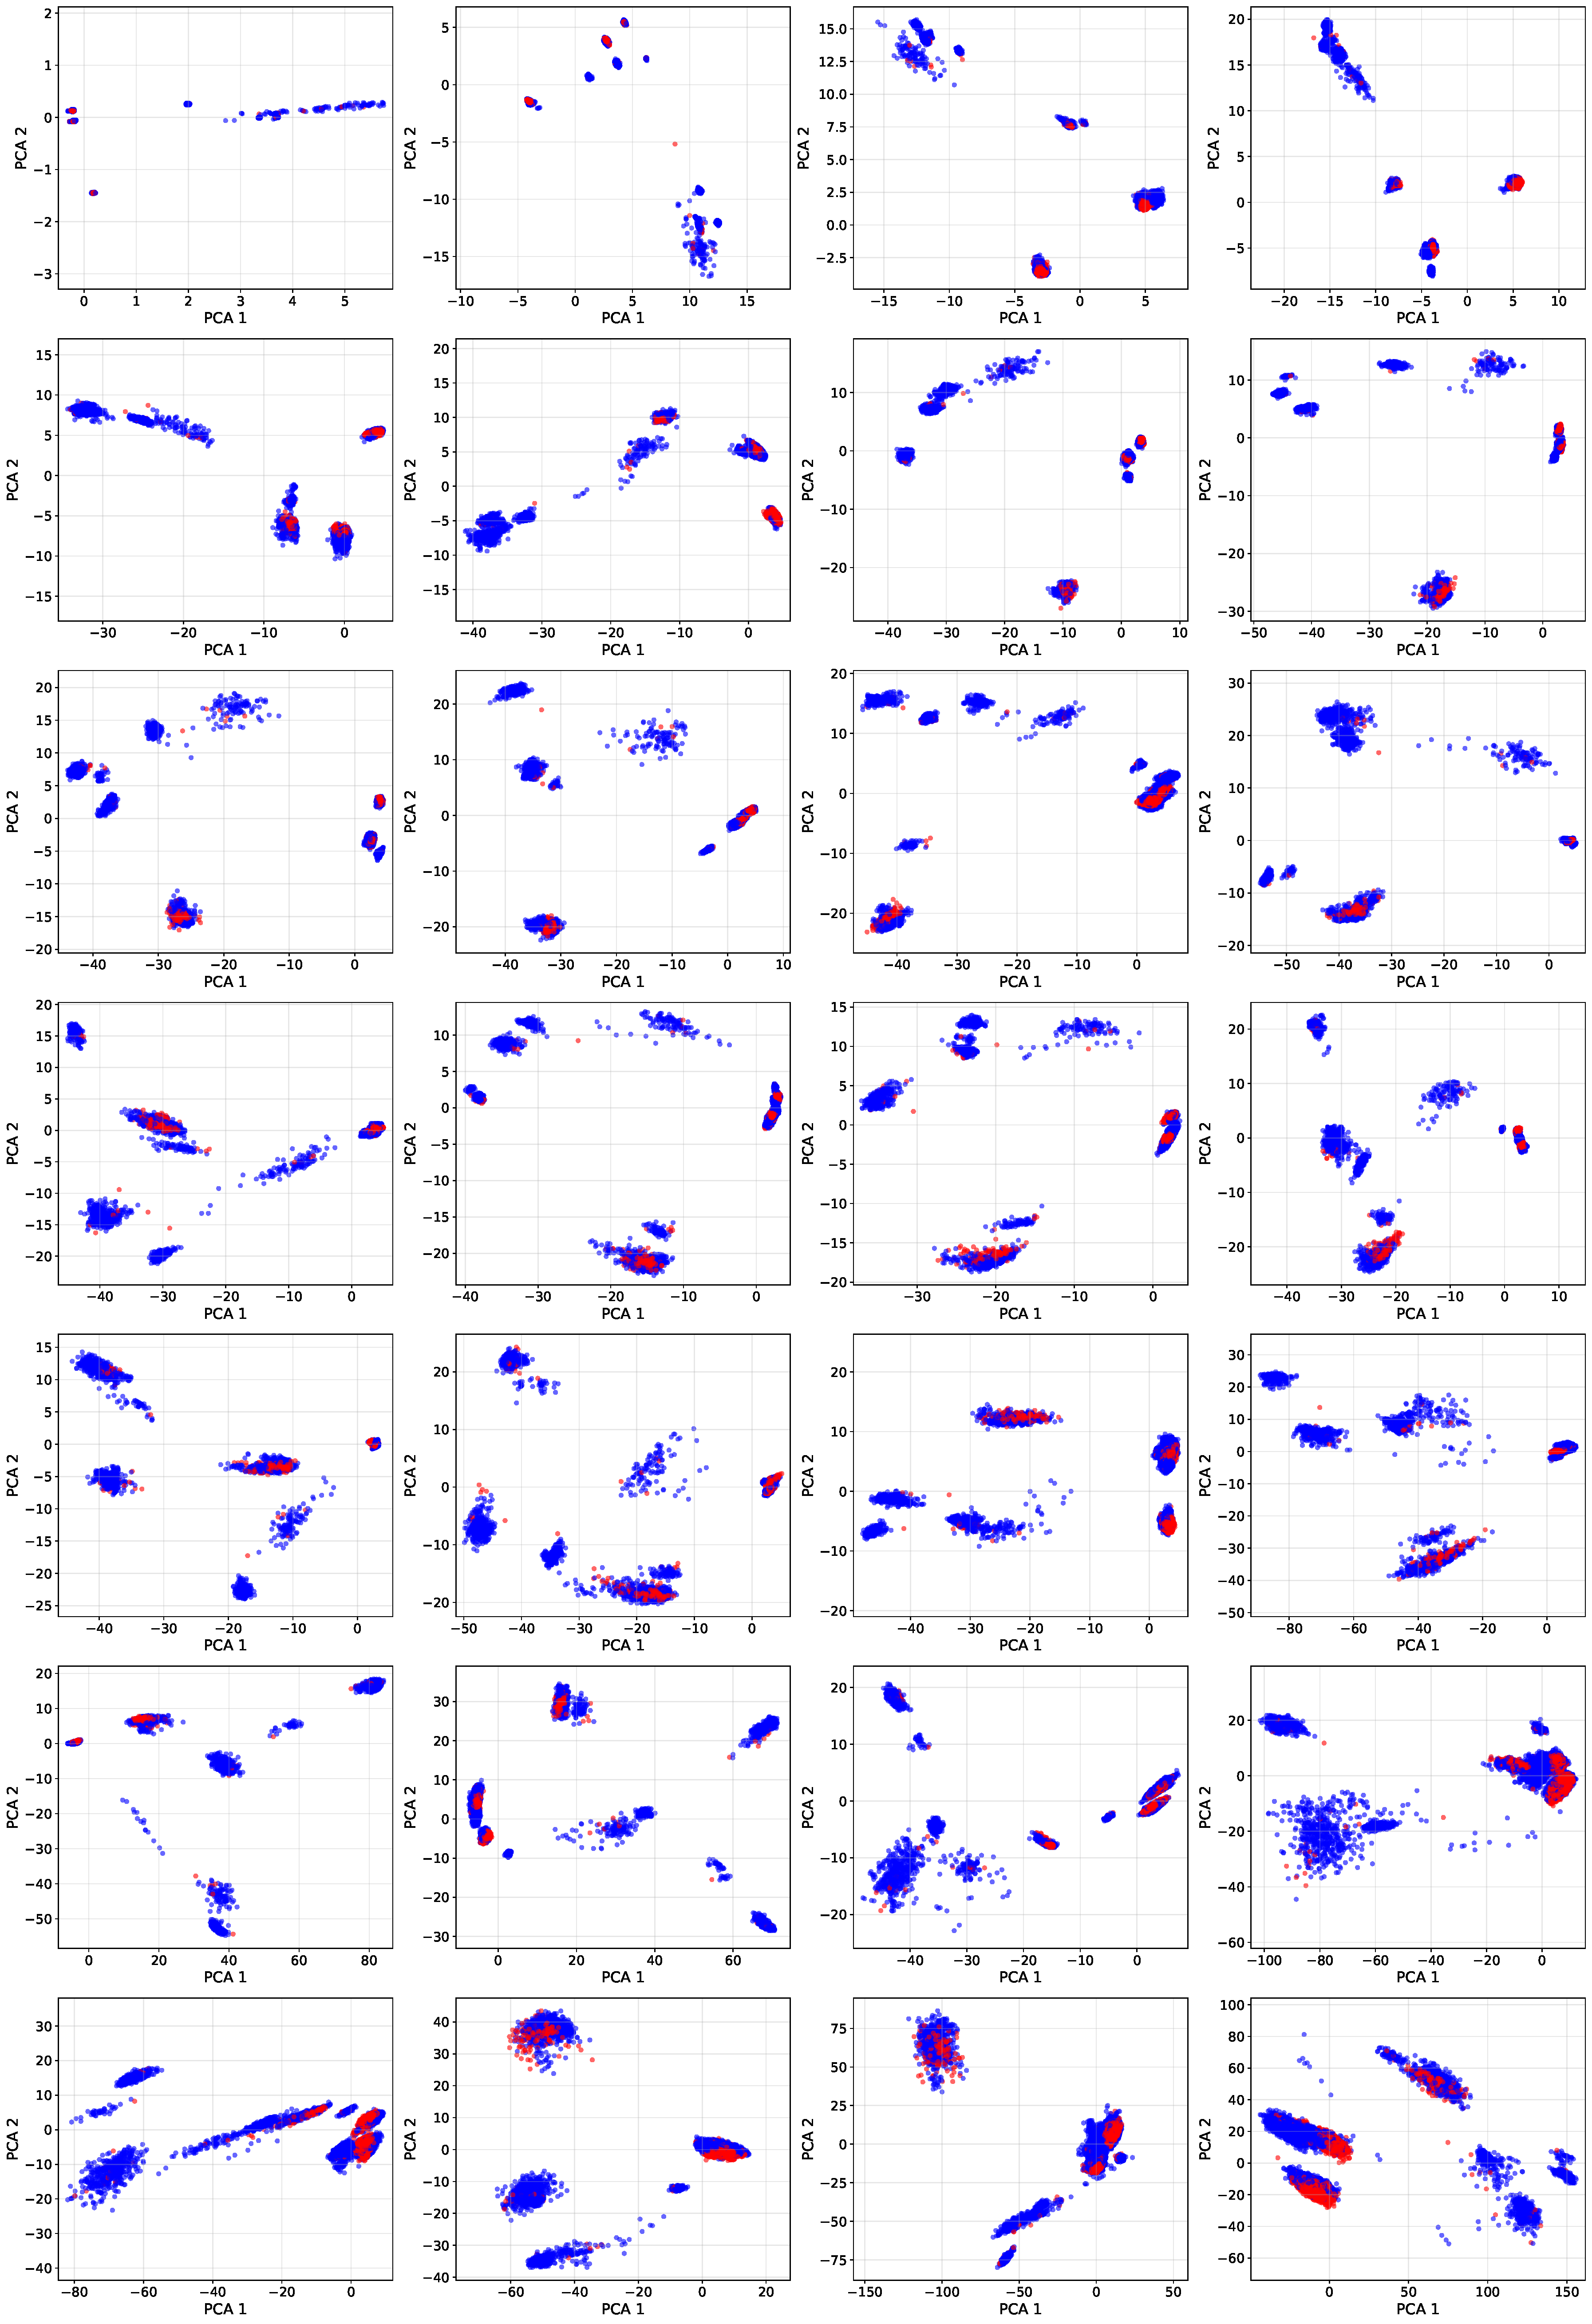
\includegraphics[width=\textwidth, height=1\textheight, keepaspectratio]{images/PCA_Plots/Falcon3-7B-Base_belief_bank_facts_attn_activations_PCA_CLEAN.pdf}
    \caption{PCA of Attention layer activations from Falcon3-7B-Base for Belief Bank Facts}

    \label{fig:falcon-pca-attn-facts-full}
\end{figure}

\begin{figure}[H]
    \centering
    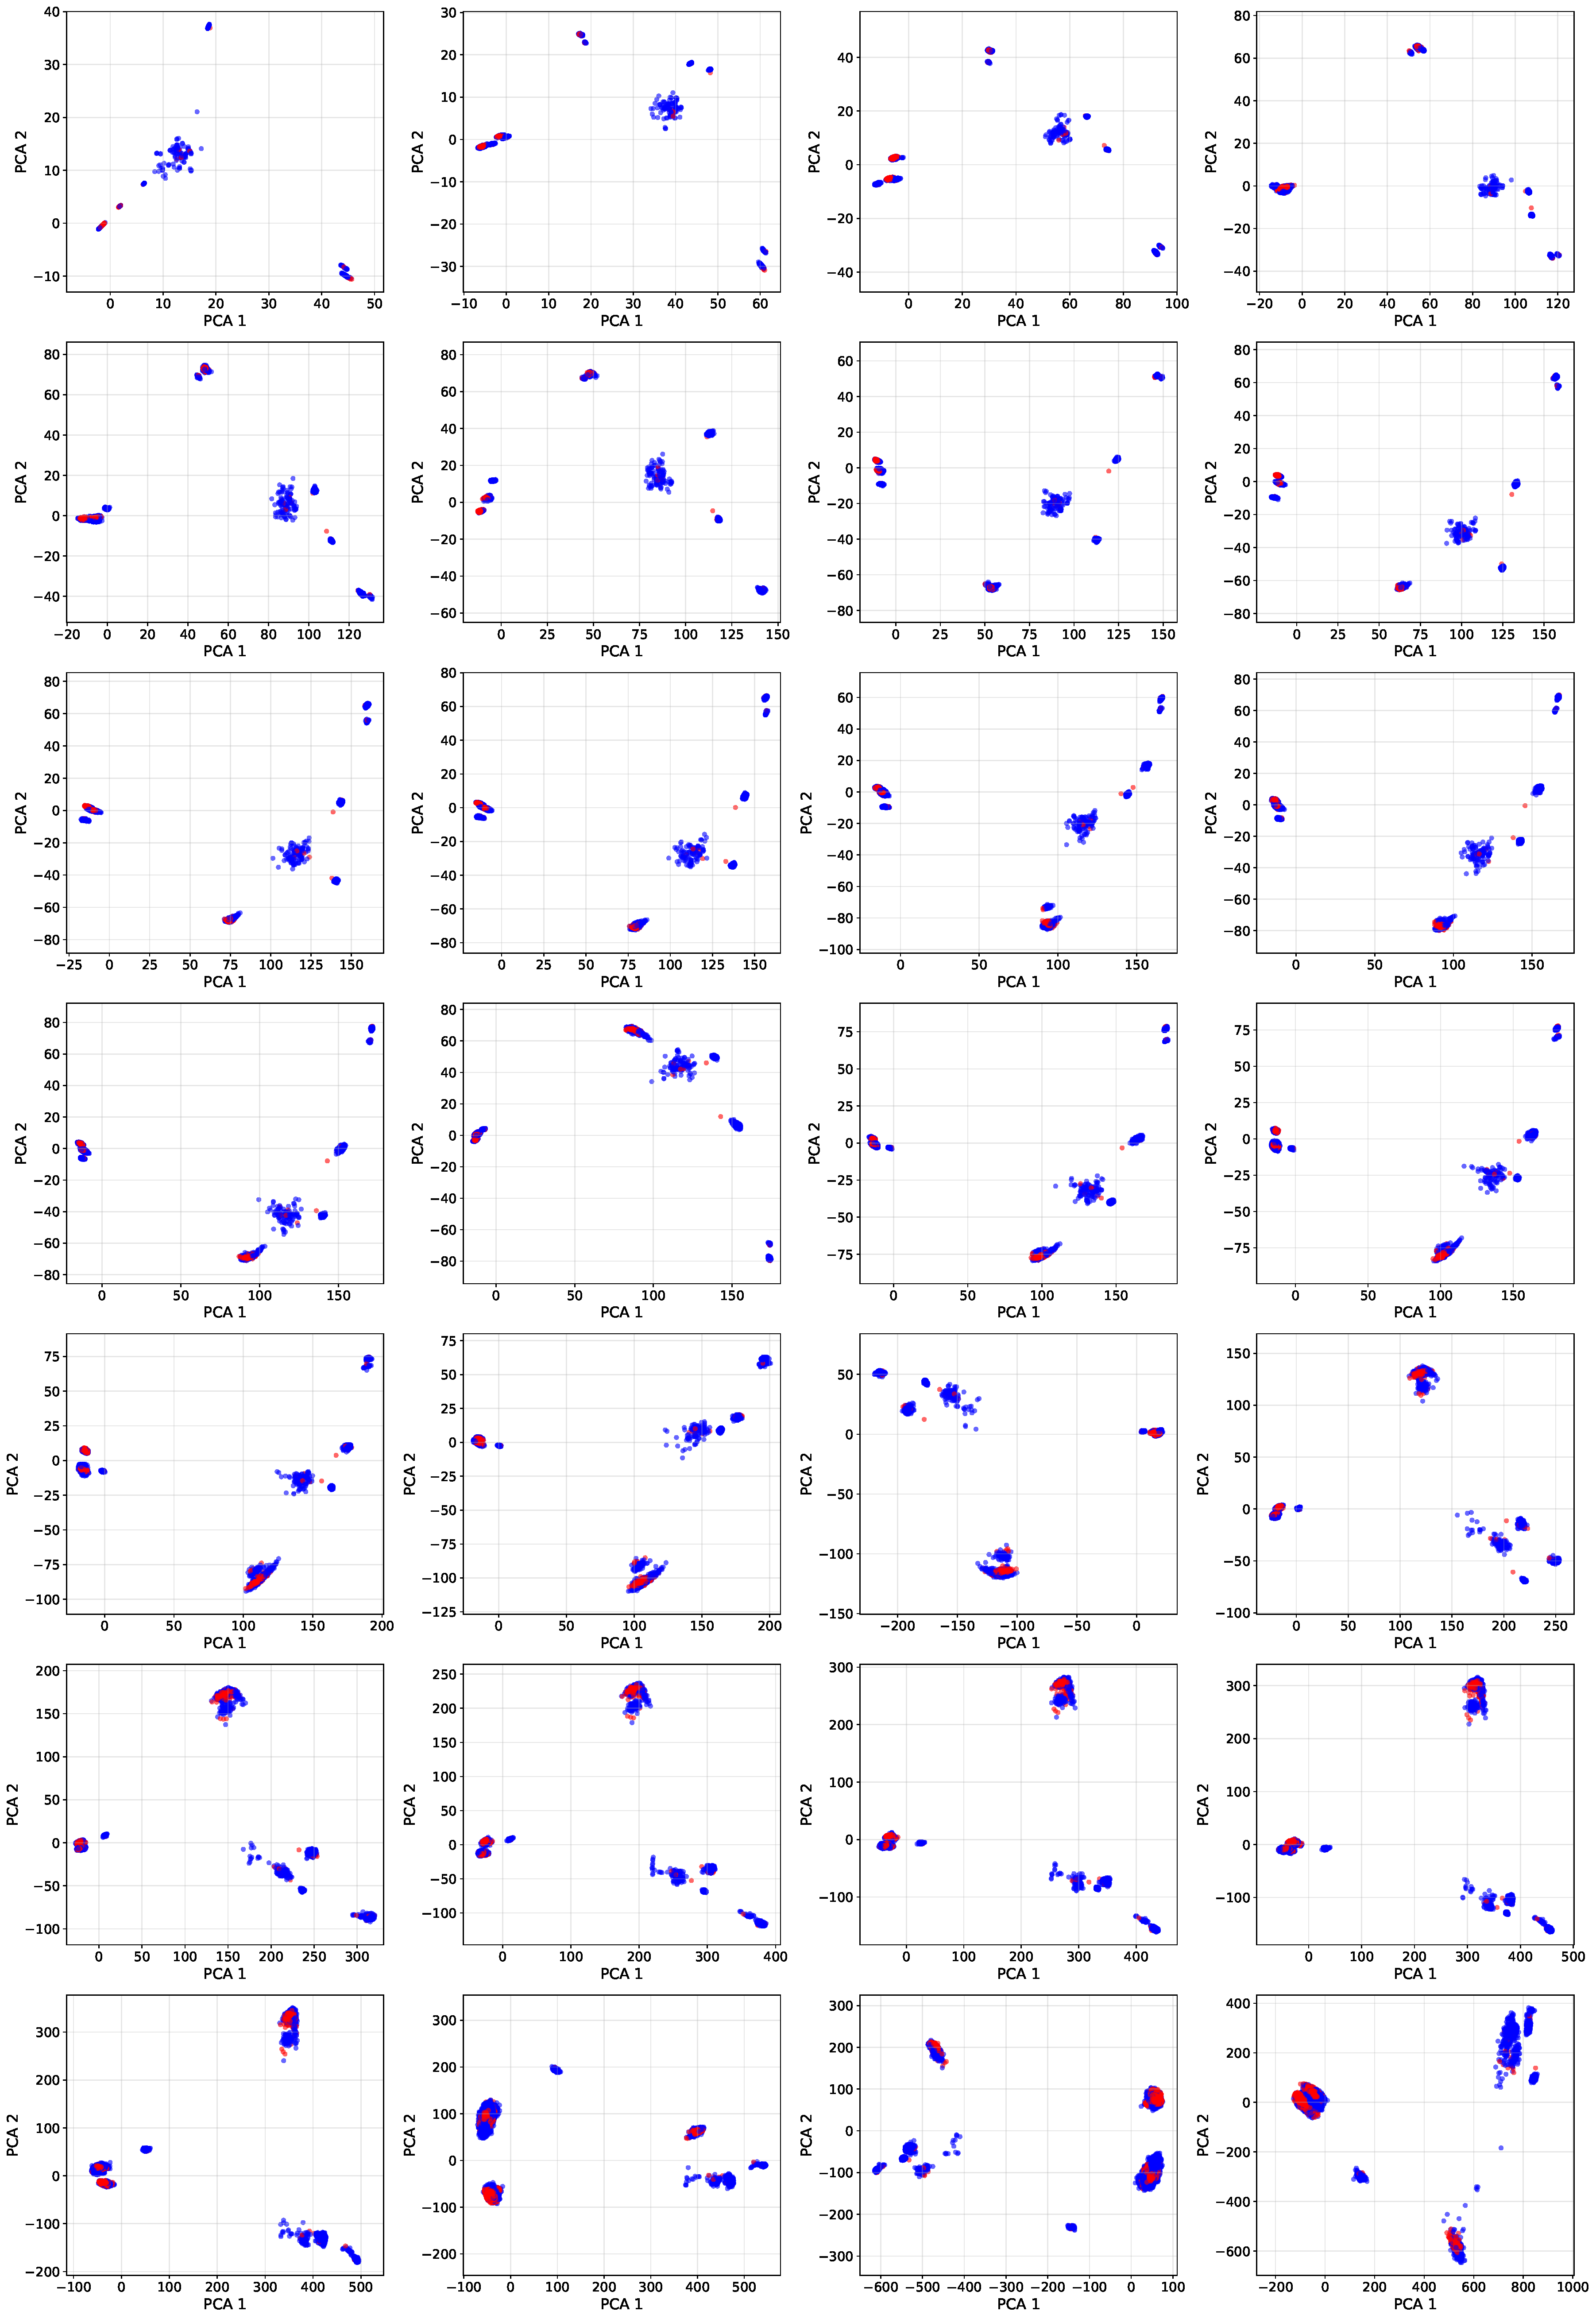
\includegraphics[width=\textwidth, height=1\textheight, keepaspectratio]{images/PCA_Plots/Falcon3-7B-Base_belief_bank_facts_hidden_activations_PCA_CLEAN.pdf}
    \caption{PCA of Hidden layer activations from Falcon3-7B-Base for Belief Bank Facts}

    \label{fig:falcon-pca-hidden-facts-full}
\end{figure}

\begin{figure}[H]
    \centering
    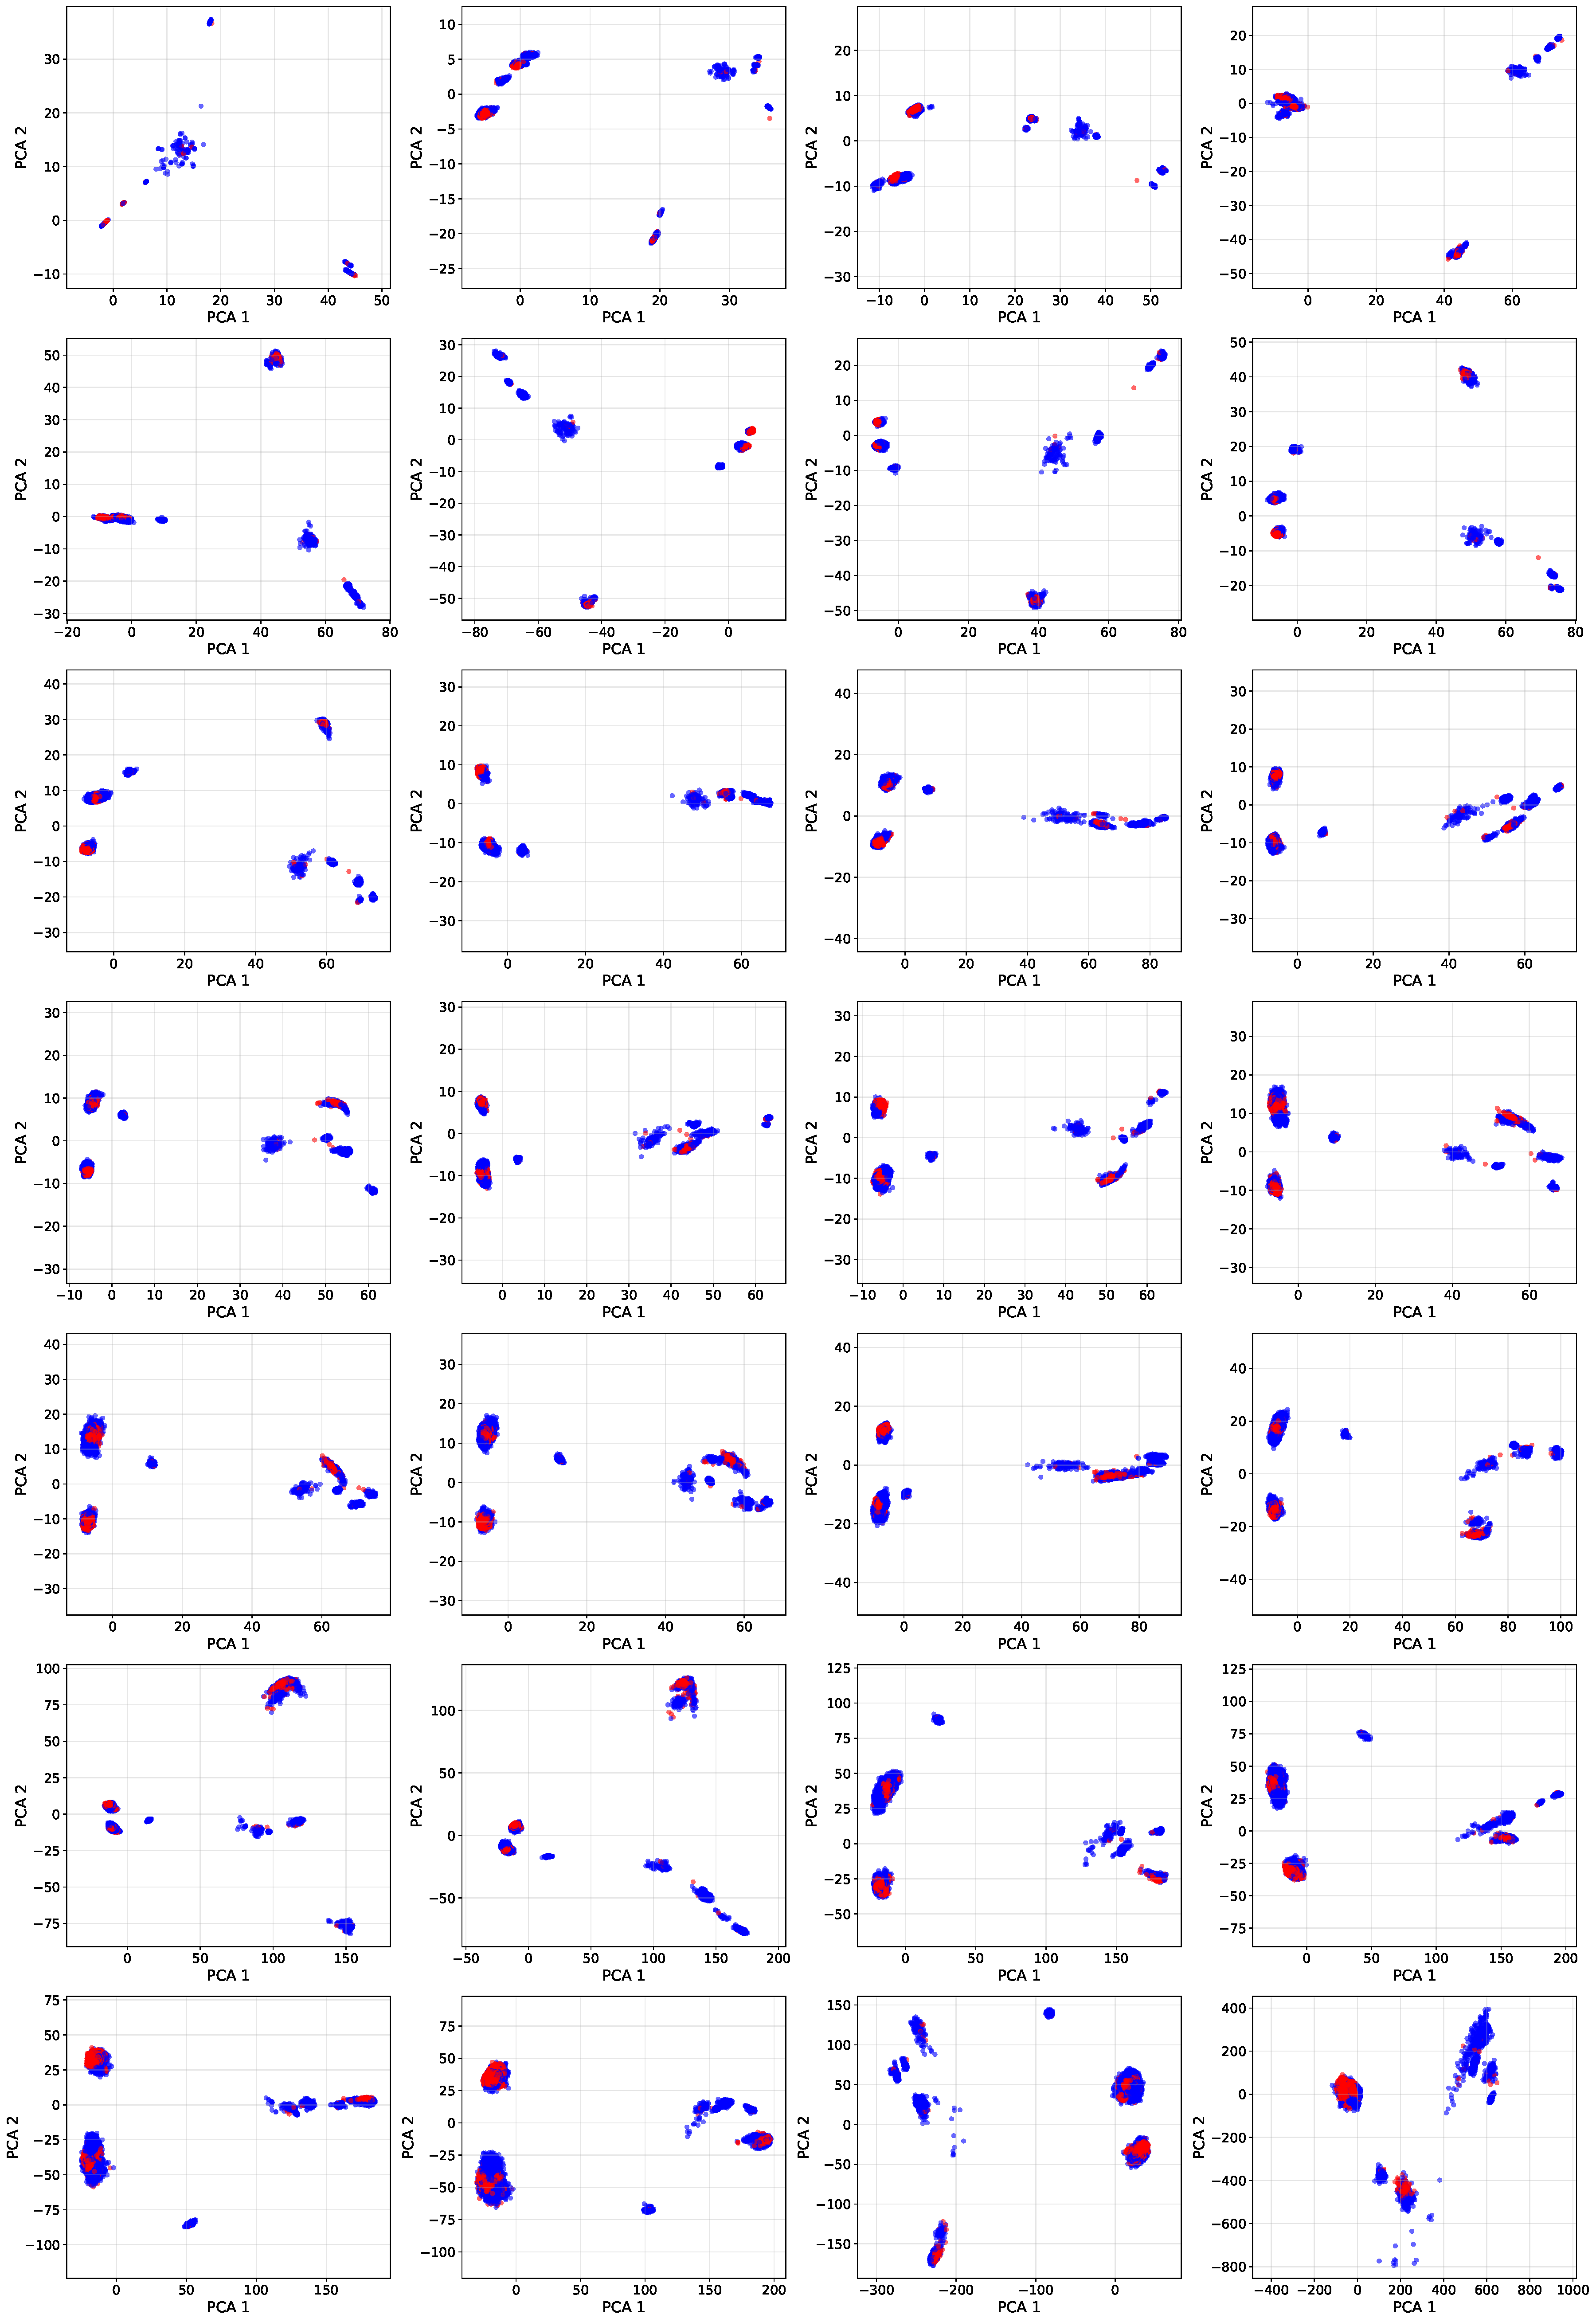
\includegraphics[width=\textwidth, height=1\textheight, keepaspectratio]{images/PCA_Plots/Falcon3-7B-Base_belief_bank_facts_mlp_activations_PCA_CLEAN.pdf}
    \caption{PCA of MLP layer activations from Falcon3-7B-Base for Belief Bank Facts}

    \label{fig:falcon-pca-mlp-facts-full}
\end{figure}


\begin{figure}[H]
    \centering
    \includegraphics[width=\textwidth, height=1\textheight, keepaspectratio]{images/PCA_Plots/gemma-2-9b-it_belief_bank_facts_attn_activations_PCA_CLEAN.pdf}
    \label{fig:gemma-pca-attn-facts-full}
    \caption{PCA of Attention layer activations from Gemma-2-9B-IT for Belief Bank Facts}
\end{figure}

\begin{figure}[H]
    \centering
    \includegraphics[width=\textwidth, height=1\textheight, keepaspectratio]{images/PCA_Plots/gemma-2-9b-it_belief_bank_facts_hidden_activations_PCA_CLEAN.pdf}
    \label{fig:gemma-pca-hidden-facts-full}
    \caption{PCA of Hidden layer activations from Gemma-2-9B-IT for Belief Bank Facts}
\end{figure}

\begin{figure}[H]
    \centering
    \includegraphics[width=\textwidth, height=1\textheight, keepaspectratio]{images/PCA_Plots/gemma-2-9b-it_belief_bank_facts_mlp_activations_PCA_CLEAN.pdf}
    \label{fig:gemma-pca-mlp-facts-full}
    \caption{PCA of MLP layer activations from Gemma-2-9B-IT for Belief Bank Facts}
\end{figure}

\begin{figure}[H]
    \centering
    \includegraphics[width=\textwidth, height=1\textheight, keepaspectratio]{images/PCA_Plots/Llama-3.1-8B-Instruct_belief_bank_facts_attn_activations_PCA_CLEAN.pdf}
    \label{fig:llama-pca-attn-facts-full}
    \caption{PCA of Attention layer activations from Llama-3.1-8B-Instruct for Belief Bank Facts}
\end{figure}

\begin{figure}[H]
    \centering
    \includegraphics[width=\textwidth, height=1\textheight, keepaspectratio]{images/PCA_Plots/Llama-3.1-8B-Instruct_belief_bank_facts_hidden_activations_PCA_CLEAN.pdf}
    \label{fig:llama-pca-hidden-facts-full}
    \caption{PCA of Hidden layer activations from Llama-3.1-8B-Instruct for Belief Bank Facts}
\end{figure}

\begin{figure}[H]
    \centering
    \includegraphics[width=\textwidth, height=1\textheight, keepaspectratio]{images/PCA_Plots/Llama-3.1-8B-Instruct_belief_bank_facts_mlp_activations_PCA_CLEAN.pdf}
    \label{fig:llama-pca-mlp-facts-full}
    \caption{PCA of MLP layer activations from Llama-3.1-8B-Instruct for Belief Bank Facts}
\end{figure}


\begin{figure}[H]
    \centering
    \includegraphics[width=\textwidth, height=1\textheight, keepaspectratio]{images/PCA_Plots/gemma-2-9b-it_belief_bank_constraints_attn_activations_PCA_CLEAN.pdf}
    \label{fig:gemma-pca-attn-constraints-full}
    \caption{PCA of Attention layer activations from Gemma-2-9B-IT for Belief Bank Constraints}
\end{figure}

\begin{figure}[H]
    \centering
    \includegraphics[width=\textwidth, height=1\textheight, keepaspectratio]{images/PCA_Plots/gemma-2-9b-it_belief_bank_constraints_hidden_activations_PCA_CLEAN.pdf}
    \label{fig:gemma-pca-hidden-constraints-full}
    \caption{PCA of Hidden layer activations from Gemma-2-9B-IT for Belief Bank Constraints}
\end{figure}

\begin{figure}[H]
    \centering
    \includegraphics[width=\textwidth, height=1\textheight, keepaspectratio]{images/PCA_Plots/gemma-2-9b-it_belief_bank_constraints_mlp_activations_PCA_CLEAN.pdf}
    \label{fig:gemma-pca-mlp-constraints-full}
    \caption{PCA of MLP layer activations from Gemma-2-9B-IT for Belief Bank Constraints}
\end{figure}


\begin{figure}[H]
    \centering
    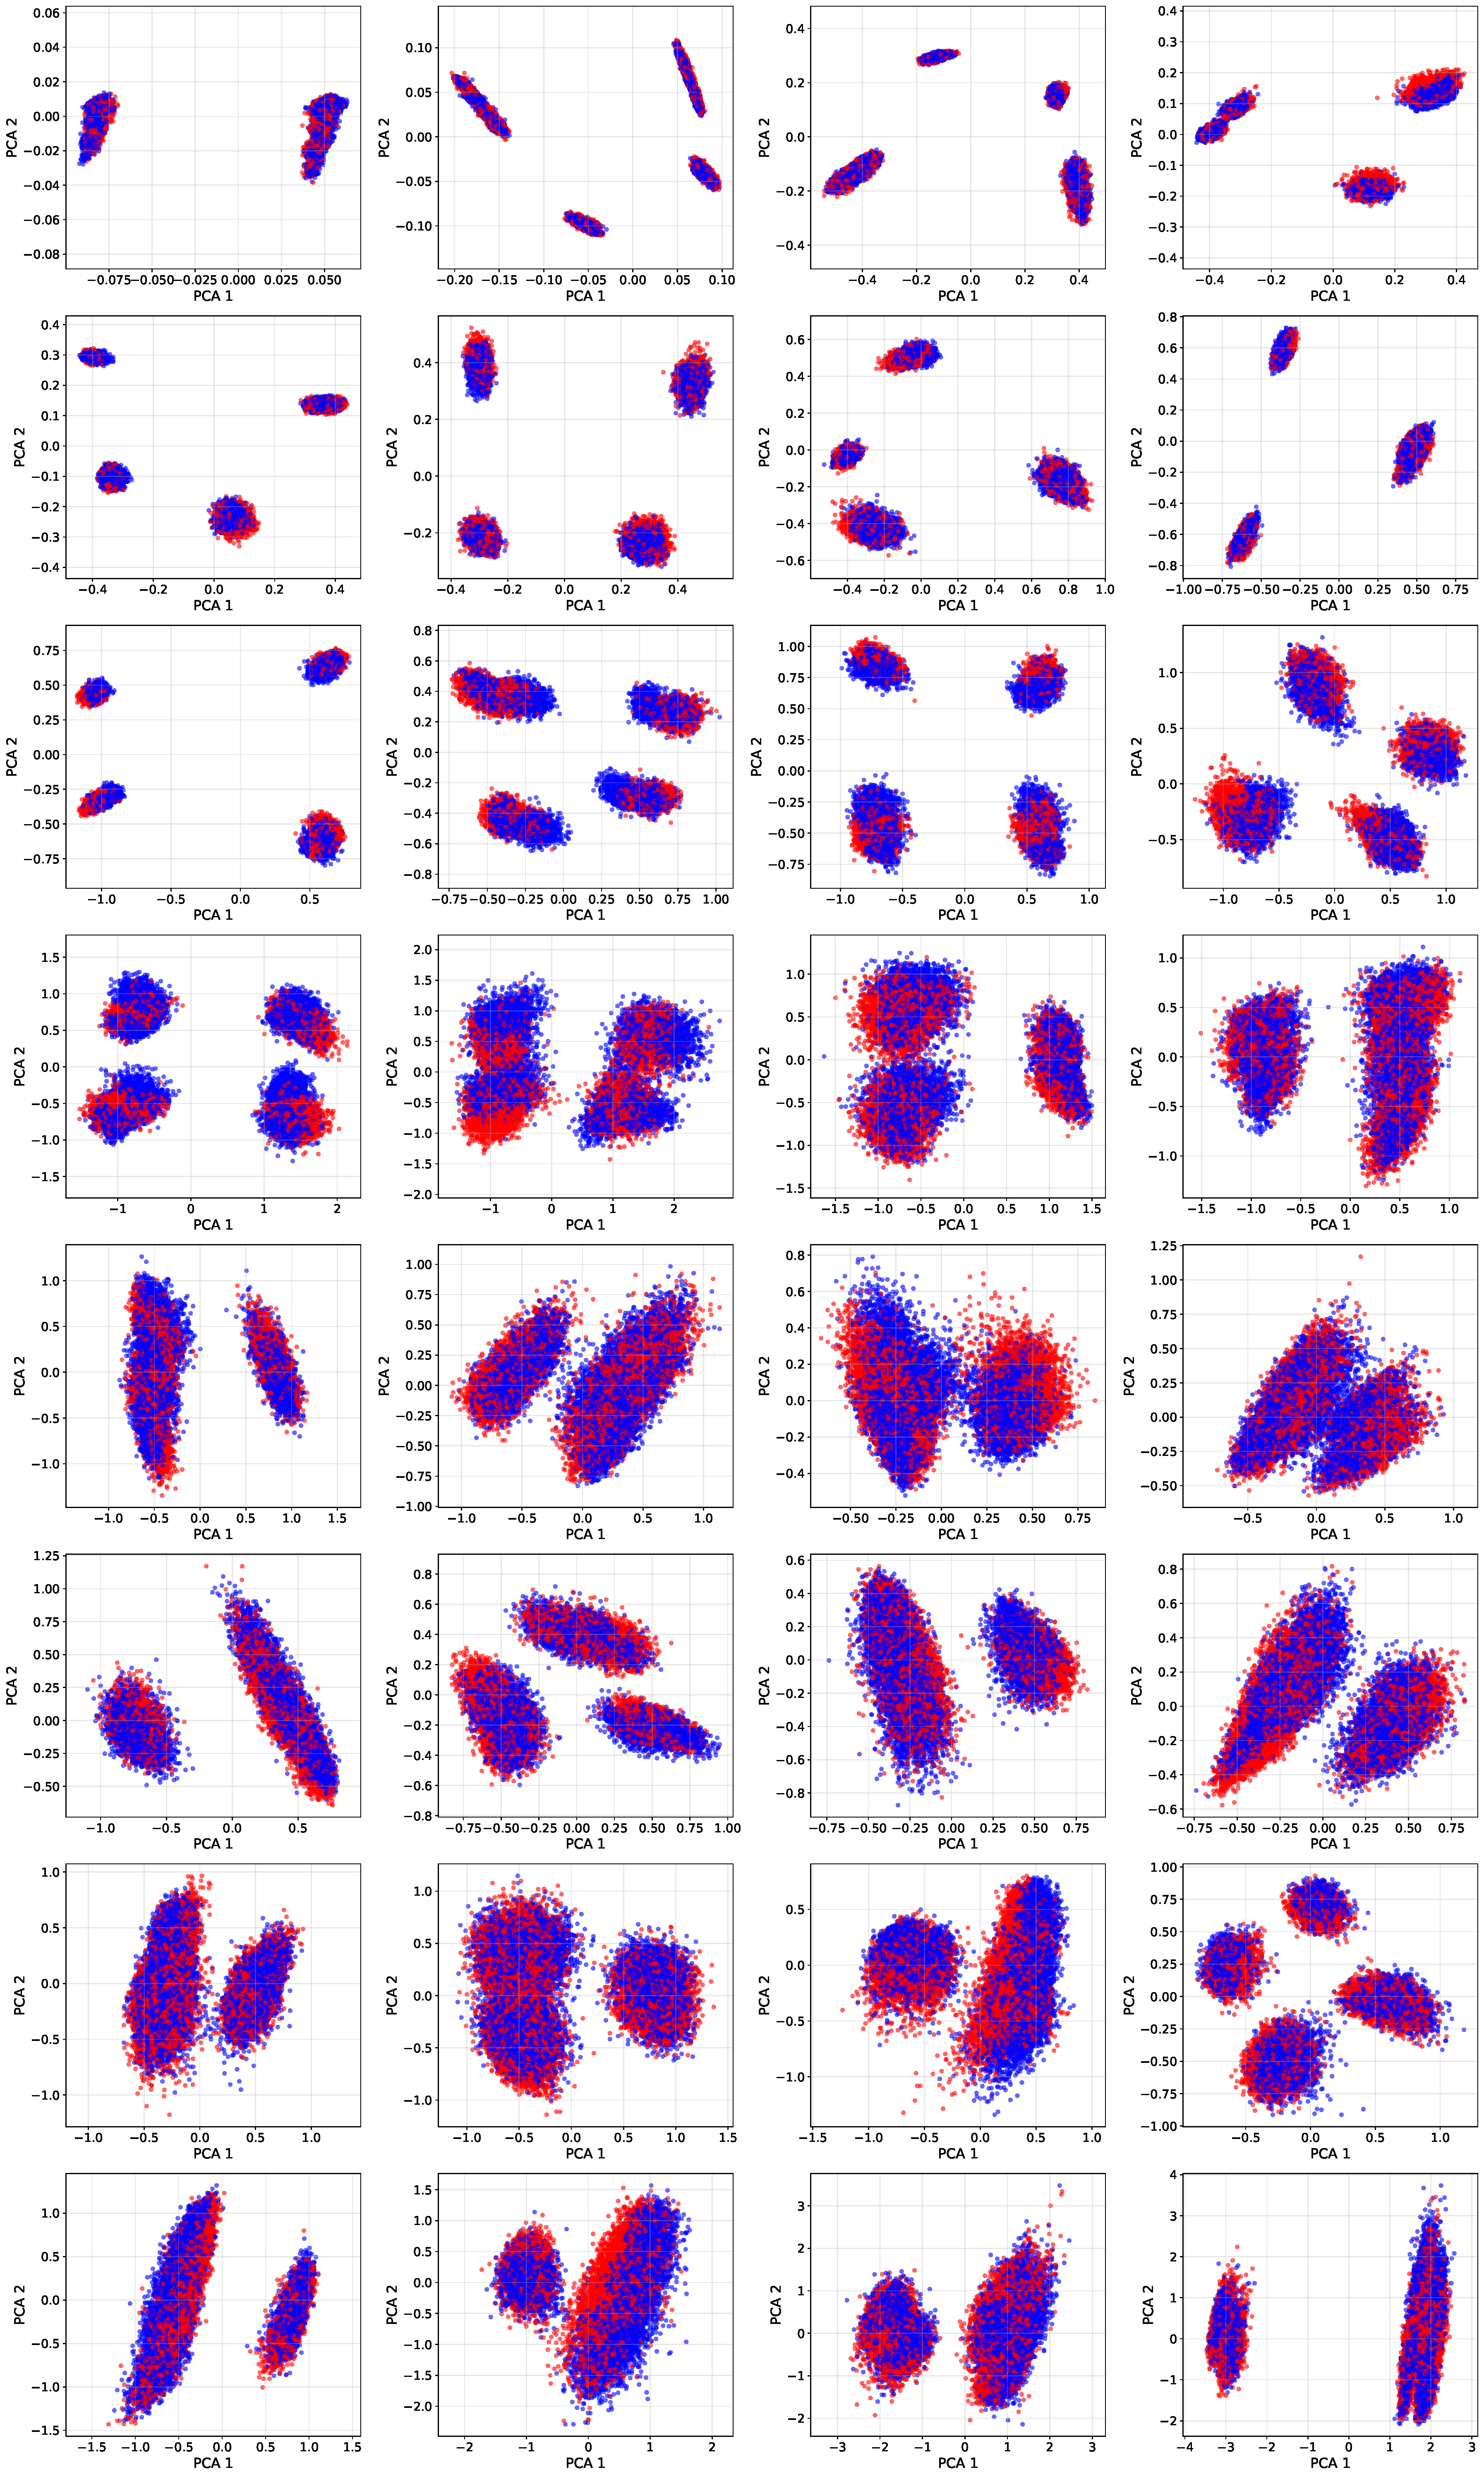
\includegraphics[width=\textwidth, height=1\textheight, keepaspectratio]{images/PCA_Plots/Llama-3.1-8B-Instruct_belief_bank_constraints_attn_activations_PCA_CLEAN.pdf}
    \label{fig:llama-pca-attn-constraints-full}
    \caption{PCA of Attention layer activations from Llama-3.1-8B-Instruct for Belief Bank Constraints}
\end{figure}

\begin{figure}[H]
    \centering
    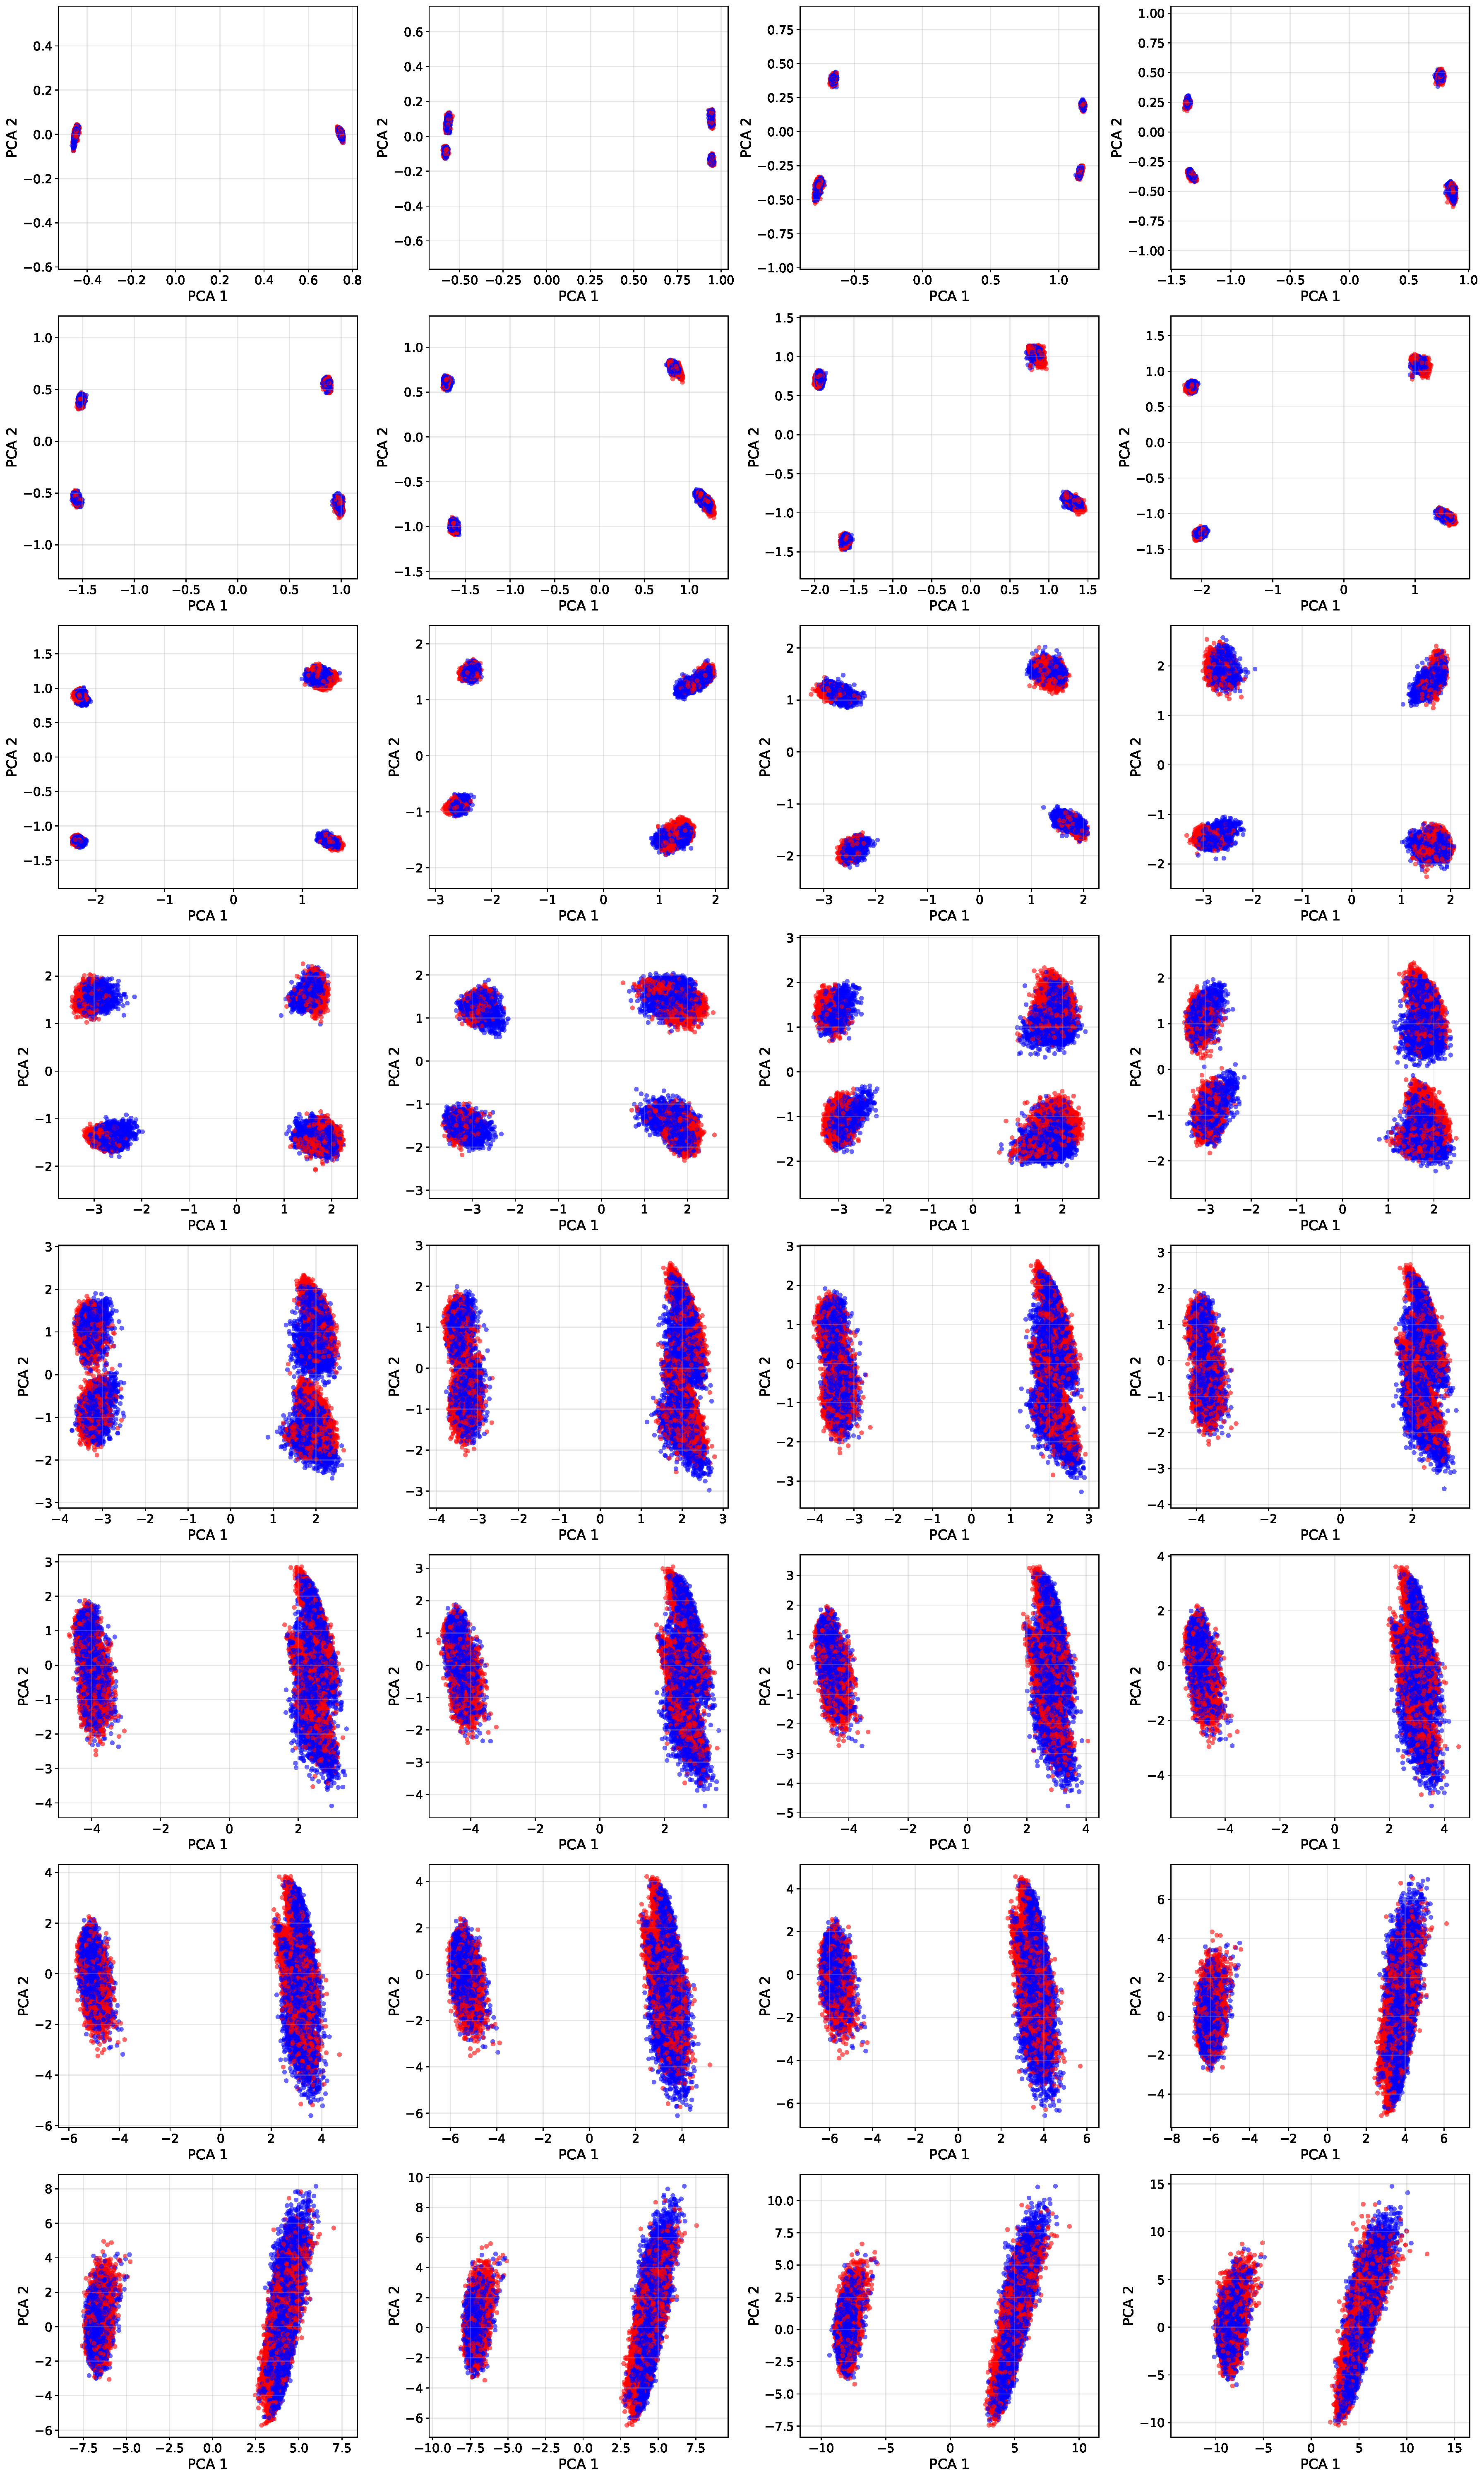
\includegraphics[width=\textwidth, height=1\textheight, keepaspectratio]{images/PCA_Plots/Llama-3.1-8B-Instruct_belief_bank_constraints_hidden_activations_PCA_CLEAN.pdf}
    \label{fig:llama-pca-hidden-constraints-full}
    \caption{PCA of Hidden layer activations from Llama-3.1-8B-Instruct for Belief Bank Constraints}
\end{figure}


\begin{figure}[H]
    \centering
    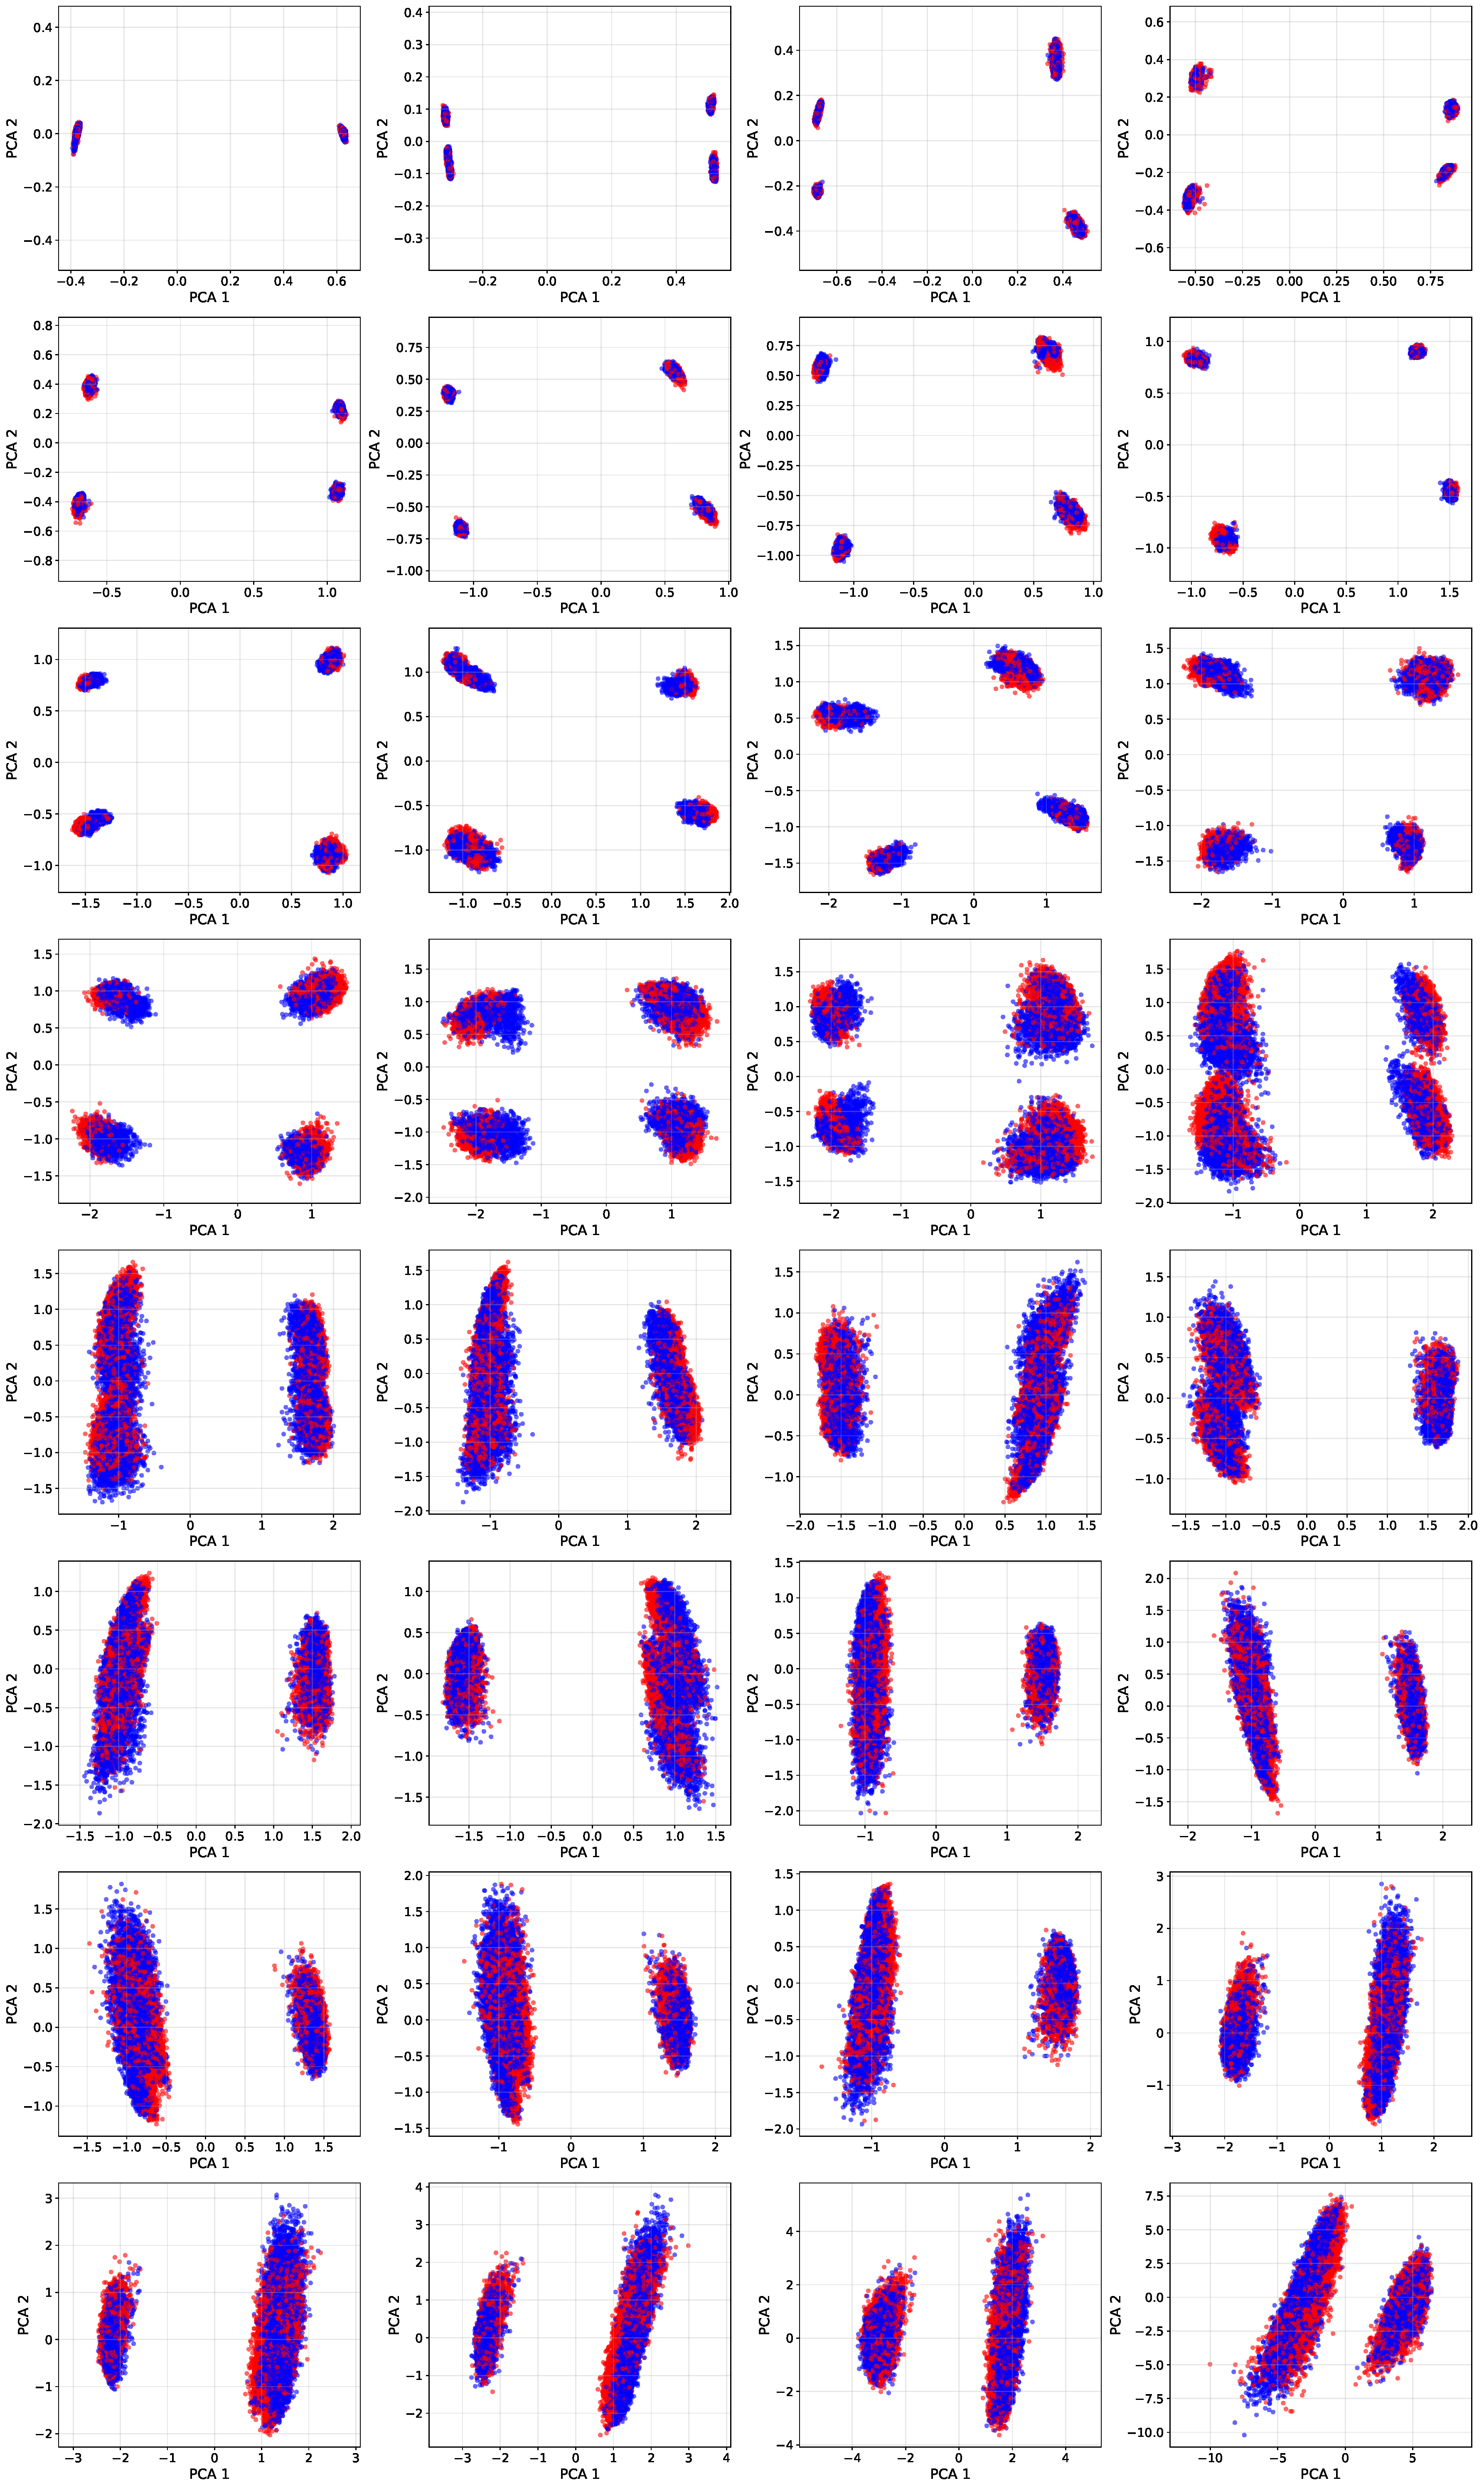
\includegraphics[width=\textwidth, height=1\textheight, keepaspectratio]{images/PCA_Plots/Llama-3.1-8B-Instruct_belief_bank_constraints_mlp_activations_PCA_CLEAN.pdf}
    \label{fig:llama-pca-mlp-constraints-full}
    \caption{PCA of MLP layer activations from Llama-3.1-8B-Instruct for Belief Bank Constraints}
\end{figure}


\begin{figure}[H]
    \centering
    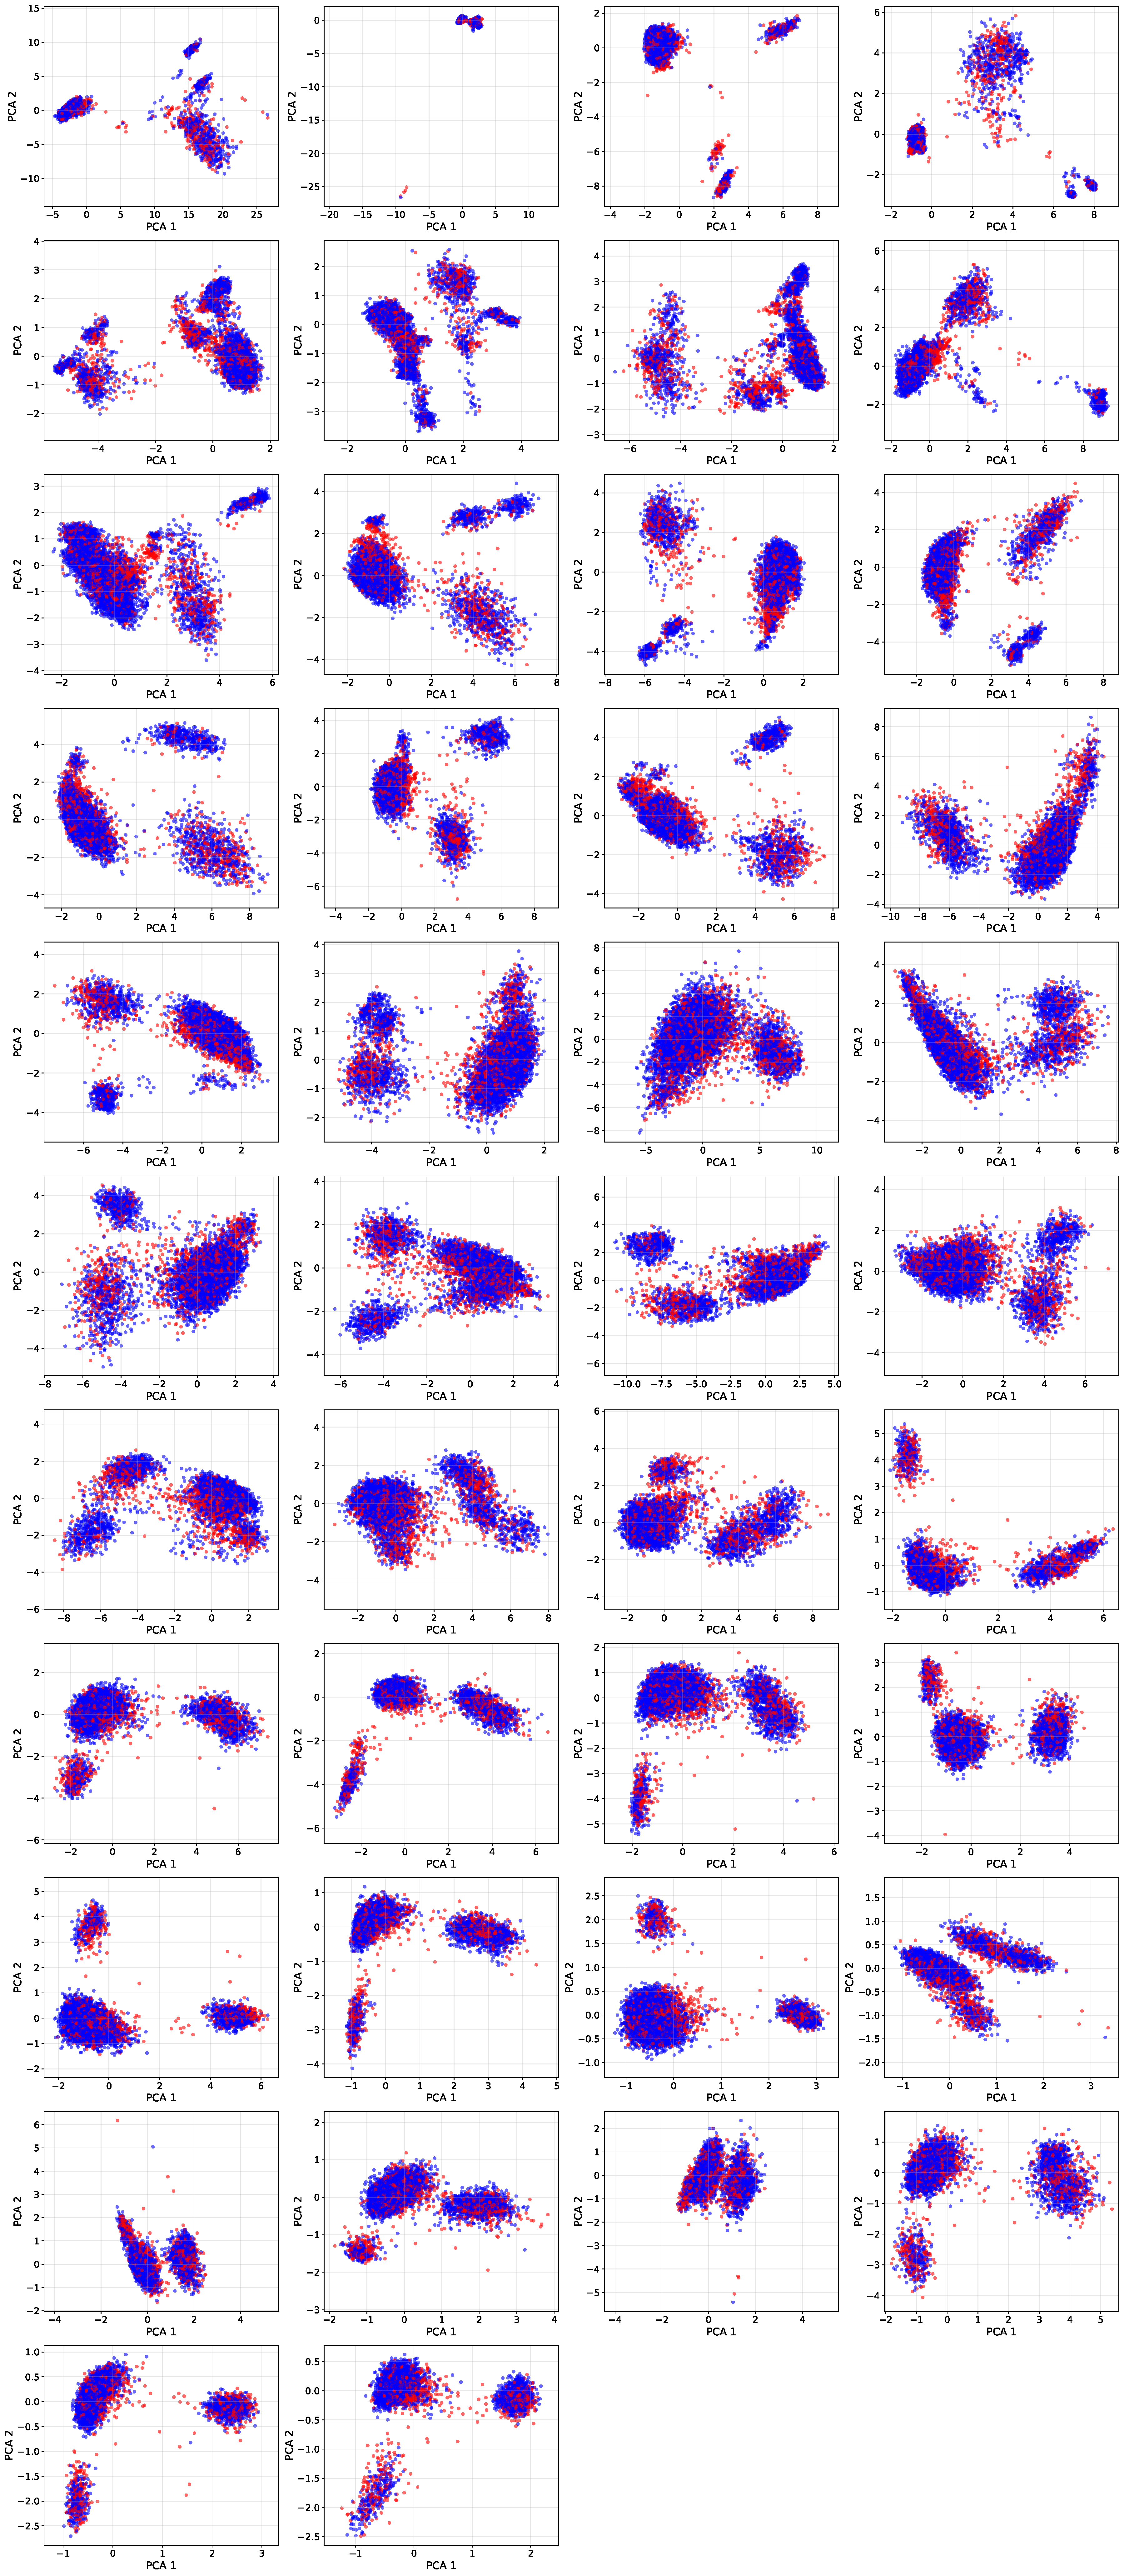
\includegraphics[width=\textwidth, height=1\textheight, keepaspectratio]{images/PCA_Plots/gemma-2-9b-it_halu_eval_attn_activations_PCA_CLEAN.pdf}
    \label{fig:gemma-pca-attn-he-full}
    \caption{PCA of Attention layer activations from Gemma-2-9B-IT for Halu Eval}
\end{figure}



\begin{figure}[H]
    \centering
    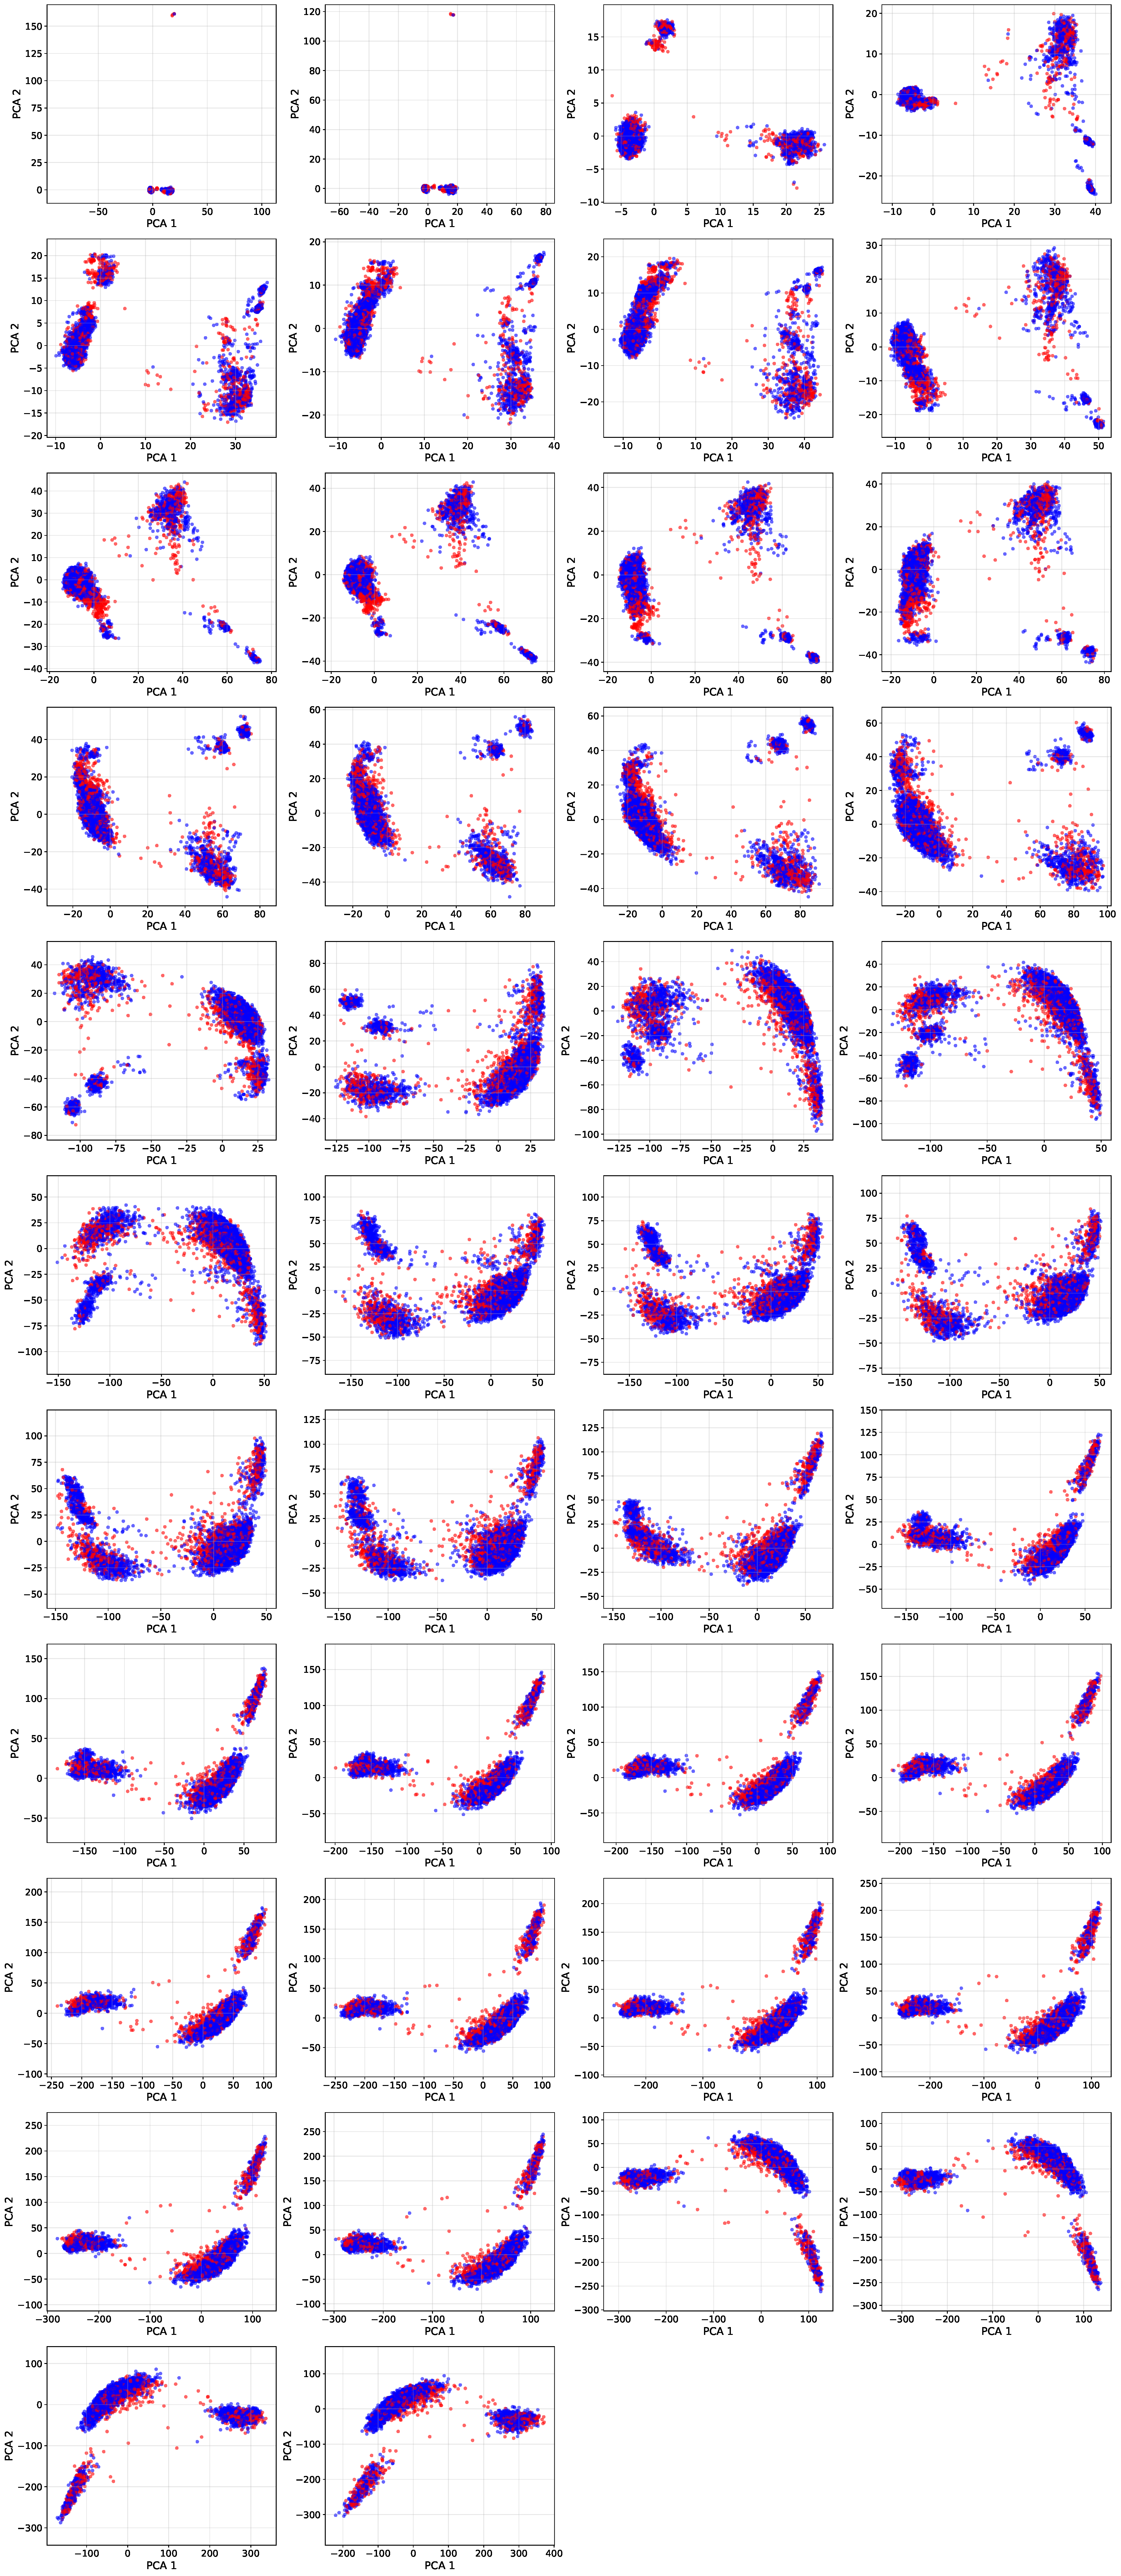
\includegraphics[width=\textwidth, height=1\textheight, keepaspectratio]{images/PCA_Plots/gemma-2-9b-it_halu_eval_hidden_activations_PCA_CLEAN.pdf}
    \label{fig:gemma-pca-hidden-he-full}
    \caption{PCA of Hidden layer activations from Gemma-2-9B-IT for Halu Eval}

\end{figure}

\begin{figure}[H]
    \centering
    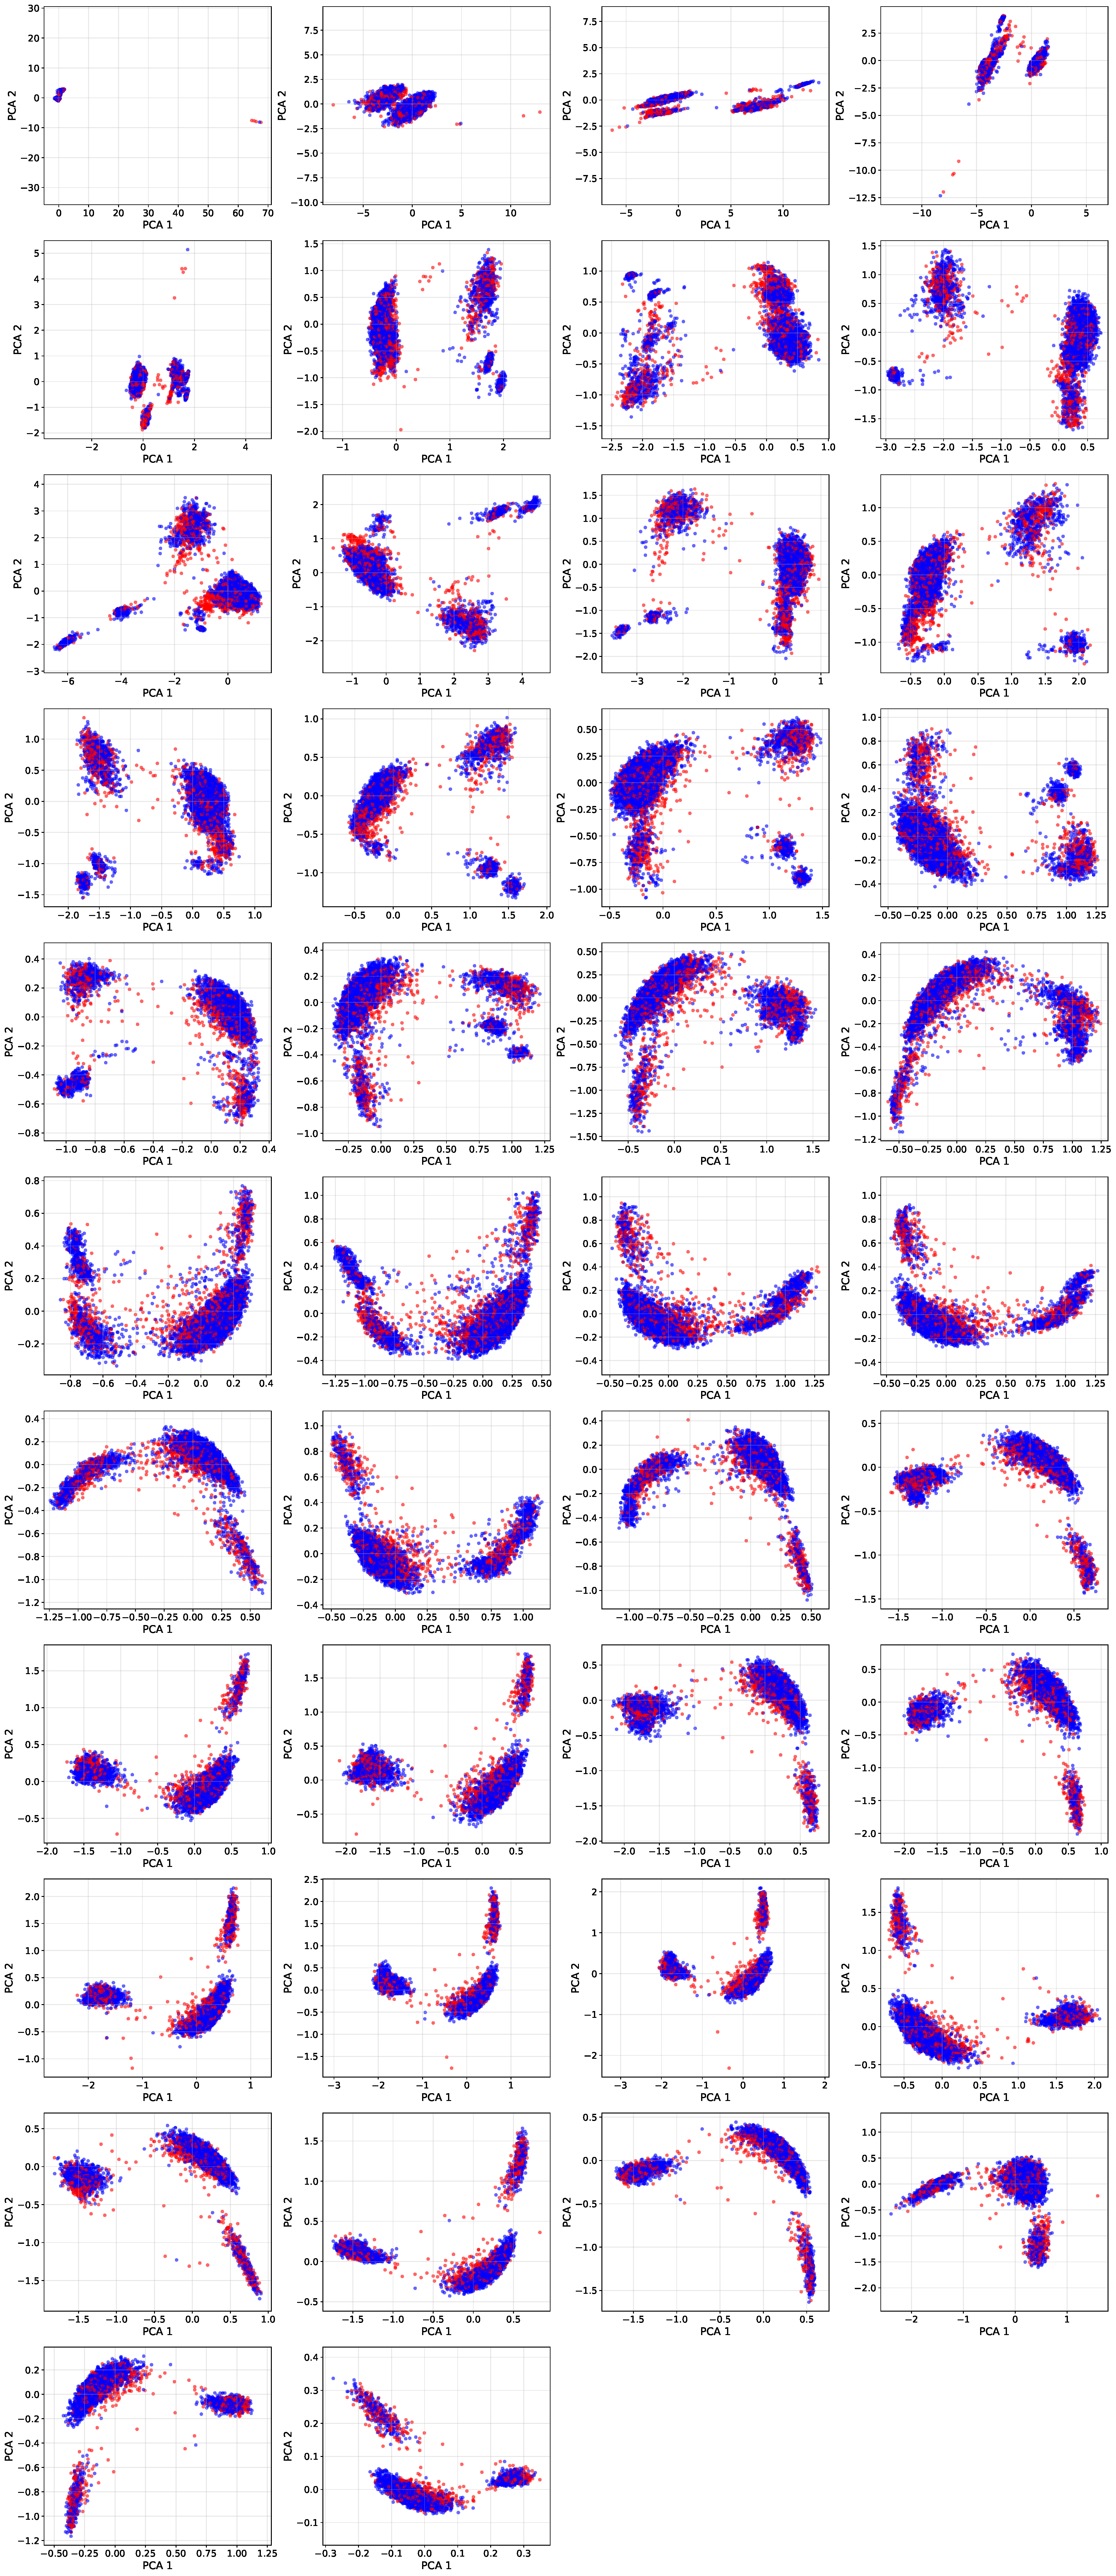
\includegraphics[width=\textwidth, height=1\textheight, keepaspectratio]{images/PCA_Plots/gemma-2-9b-it_halu_eval_mlp_activations_PCA_CLEAN.pdf}
    \label{fig:gemma-pca-mlp-he-full}
    \caption{PCA of MLP layer activations from Gemma-2-9B-IT for Halu Eval}
\end{figure}

\begin{figure}[H]
    \centering
    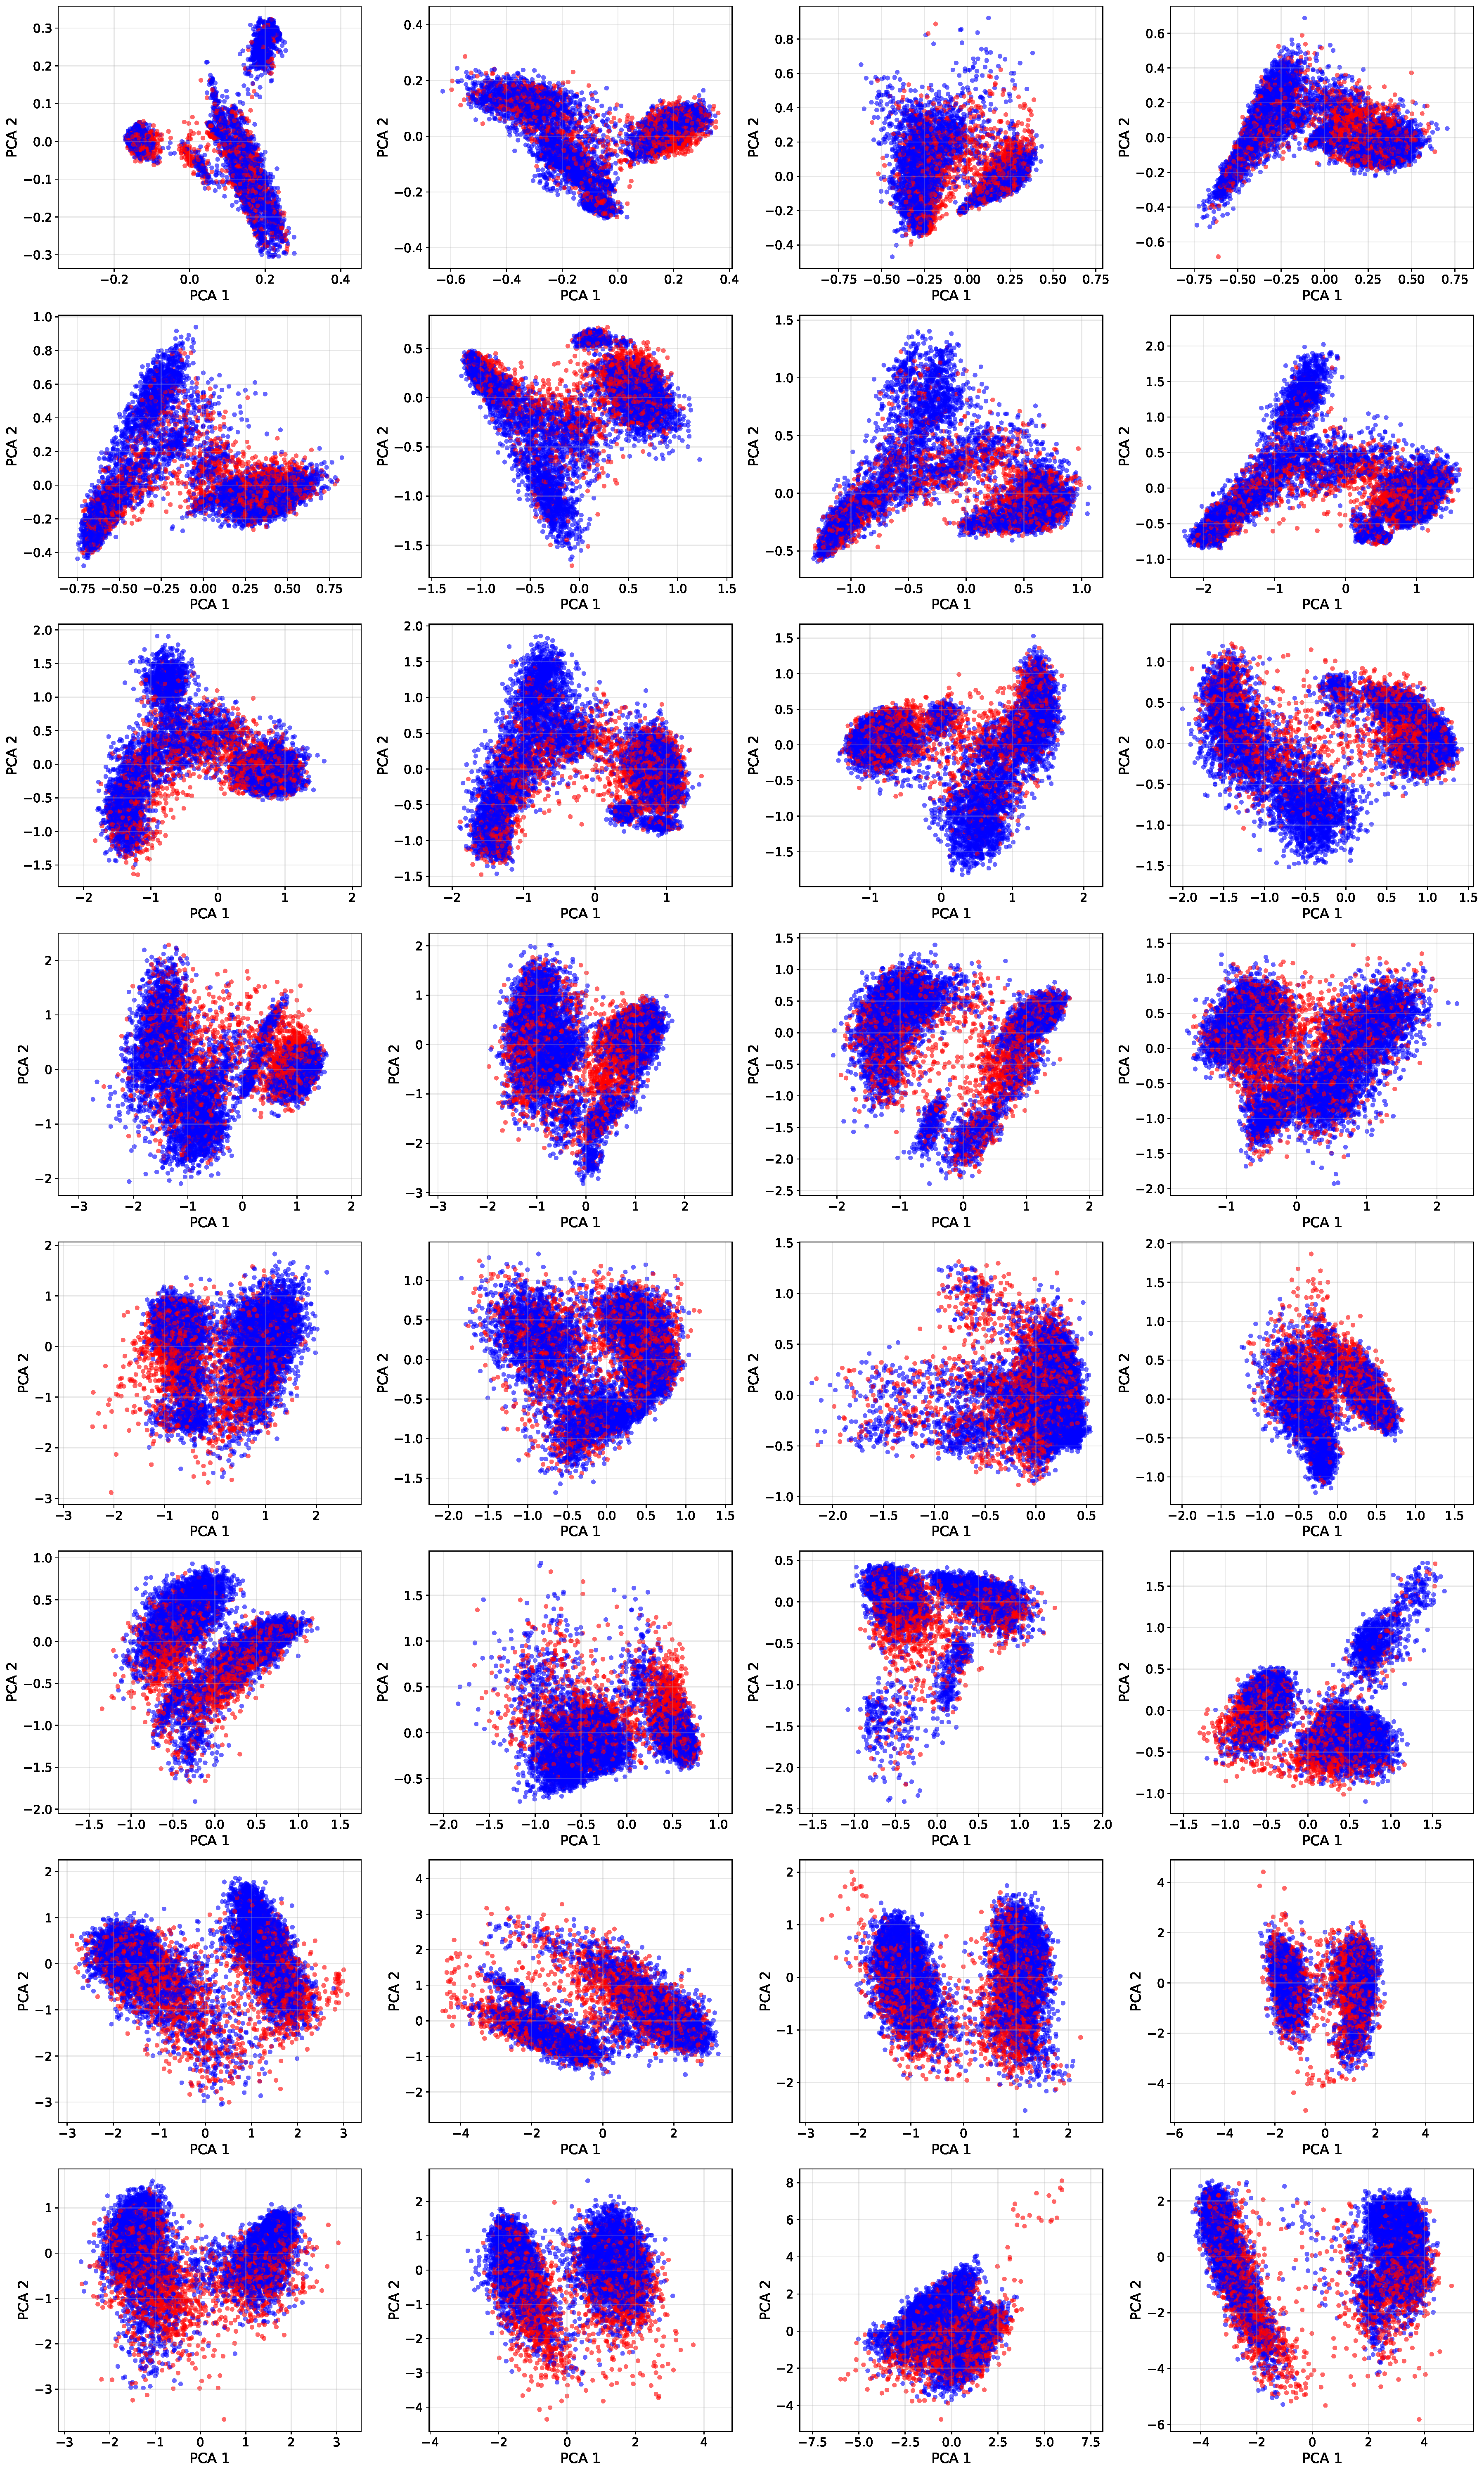
\includegraphics[width=\textwidth, height=1\textheight, keepaspectratio]{images/PCA_Plots/Llama-3.1-8B-Instruct_halu_eval_attn_activations_PCA_CLEAN.pdf}
    \label{fig:llama-pca-attn-he-full}
    \caption{PCA of Attention layer activations from Llama-3.1-8B-Instruct for Halu Eval}
\end{figure}

\begin{figure}[H]
    \centering
    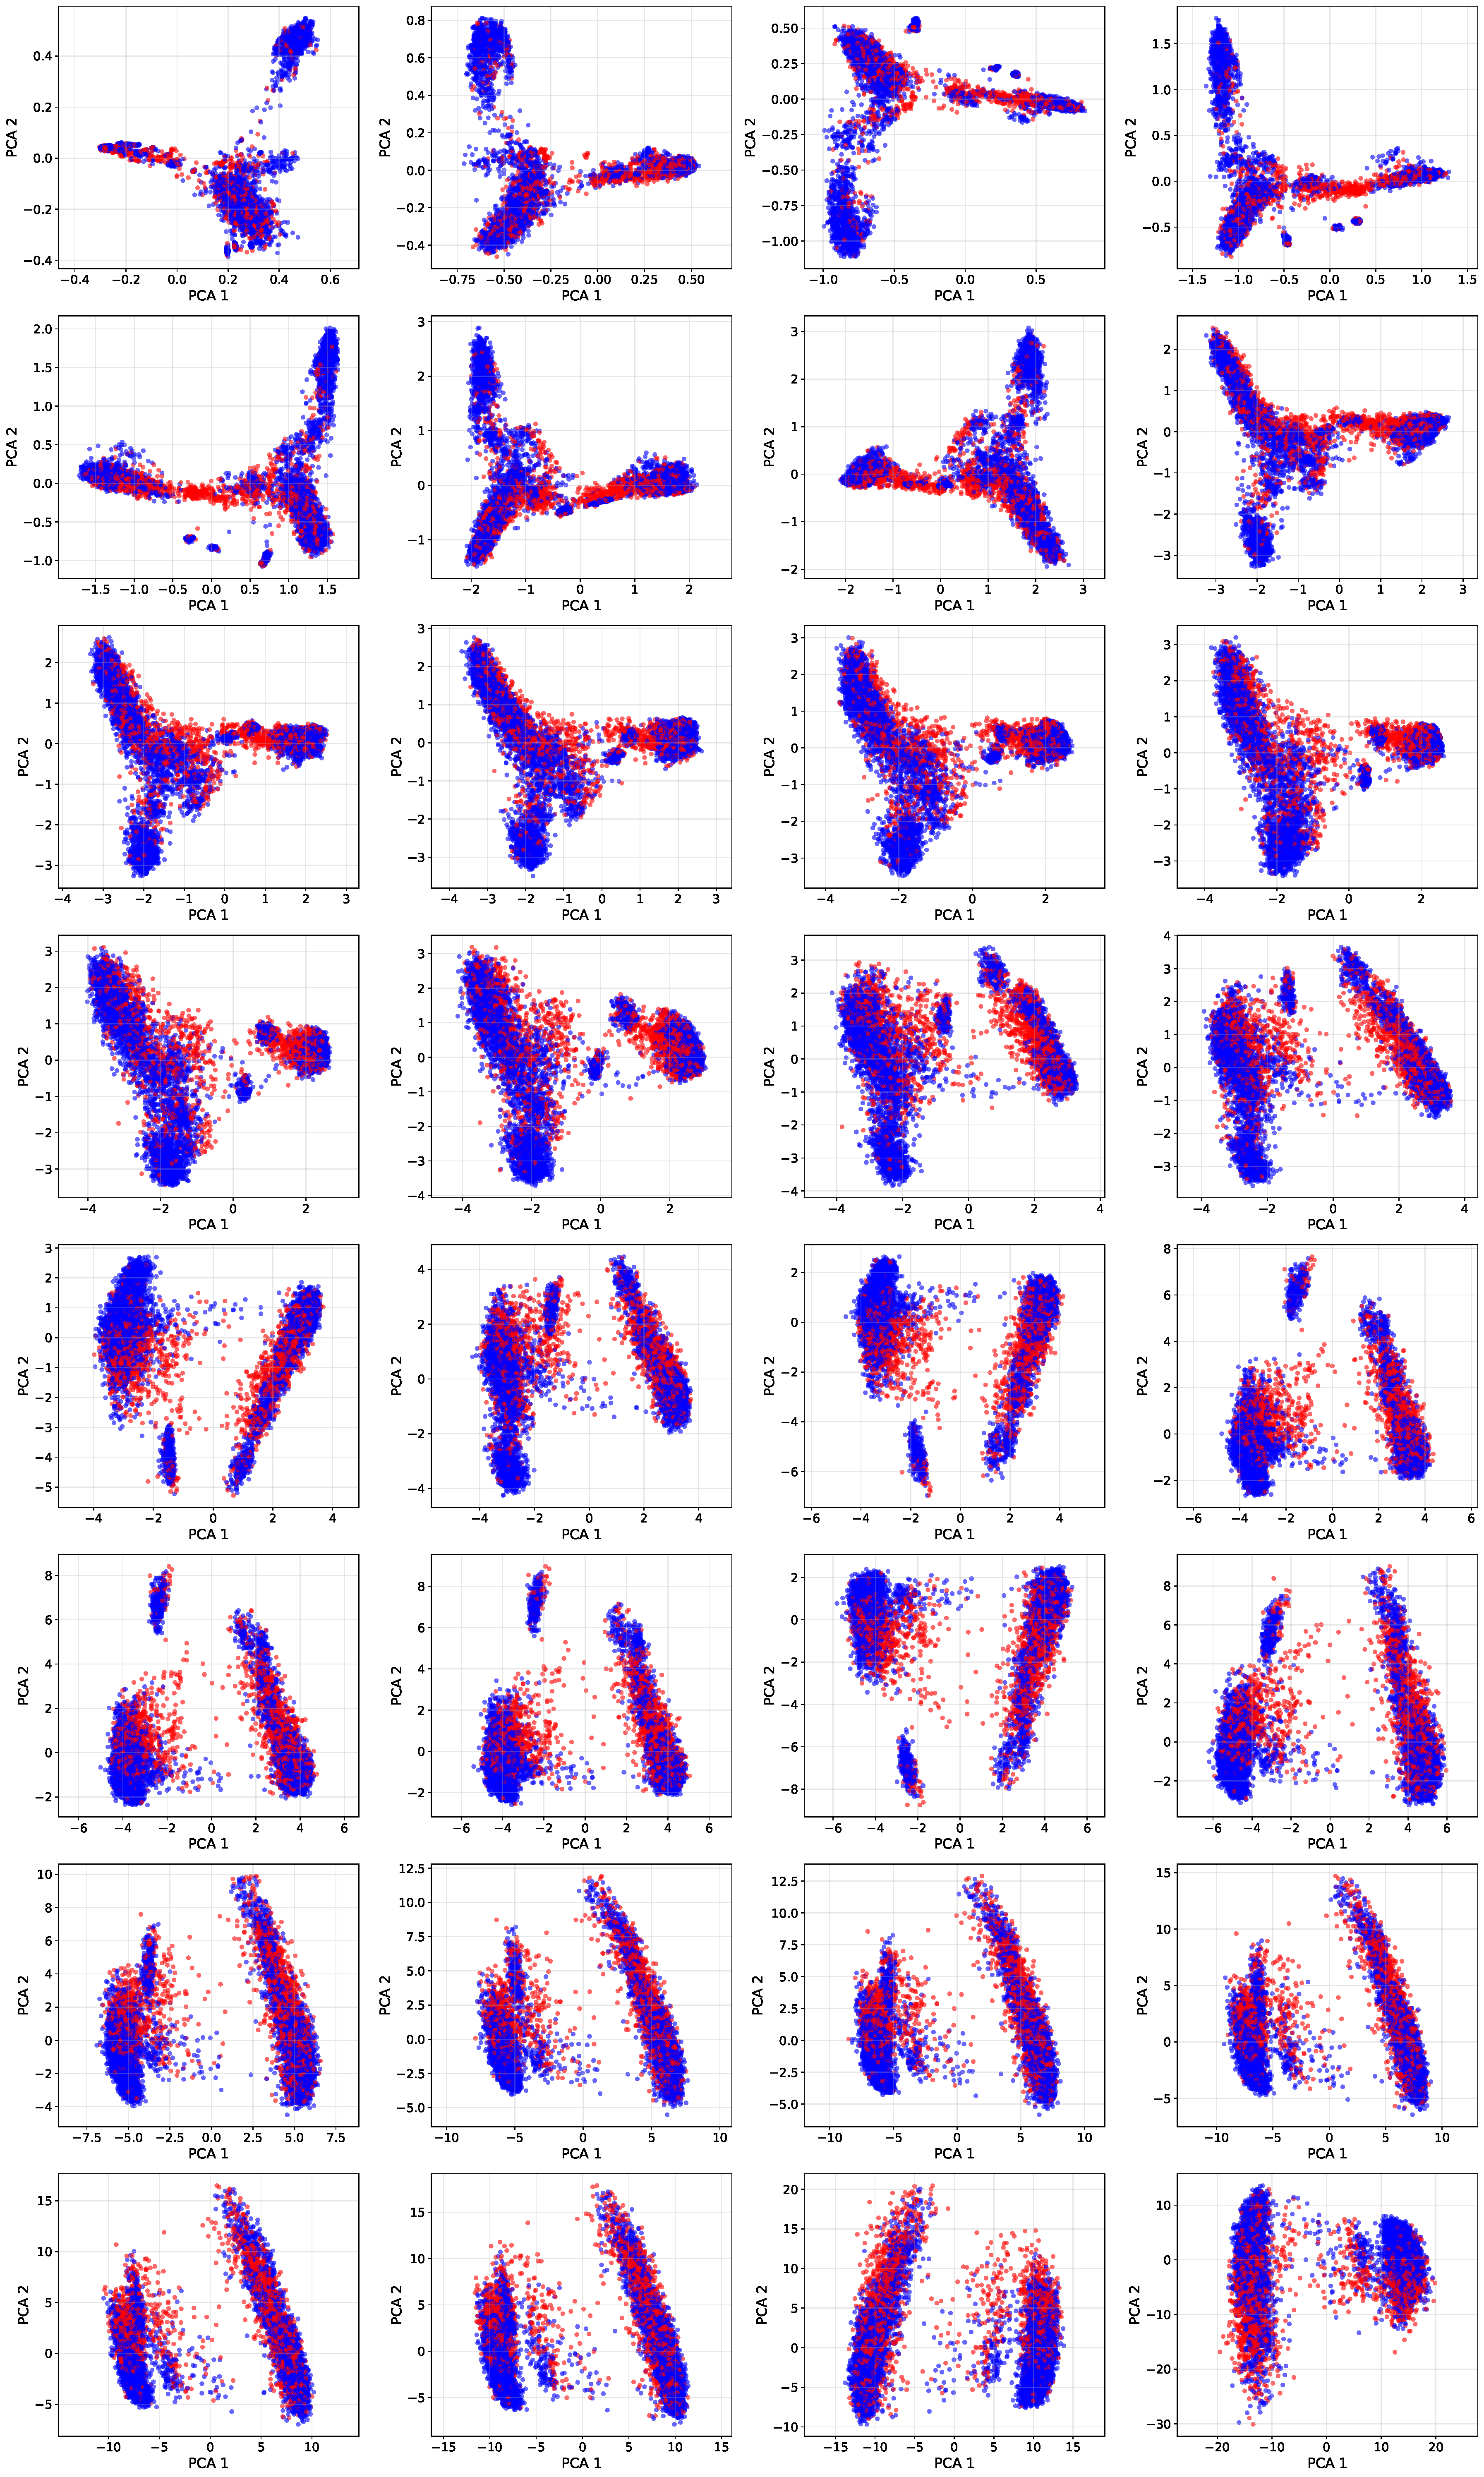
\includegraphics[width=\textwidth, height=1\textheight, keepaspectratio]{images/PCA_Plots/Llama-3.1-8B-Instruct_halu_eval_hidden_activations_PCA_CLEAN.pdf}
    \label{fig:llama-pca-hidden-he-full}
    \caption{PCA of Hidden layer activations from Llama-3.1-8B-Instruct for Halu Eval}
\end{figure}

\begin{figure}[H]
    \centering
    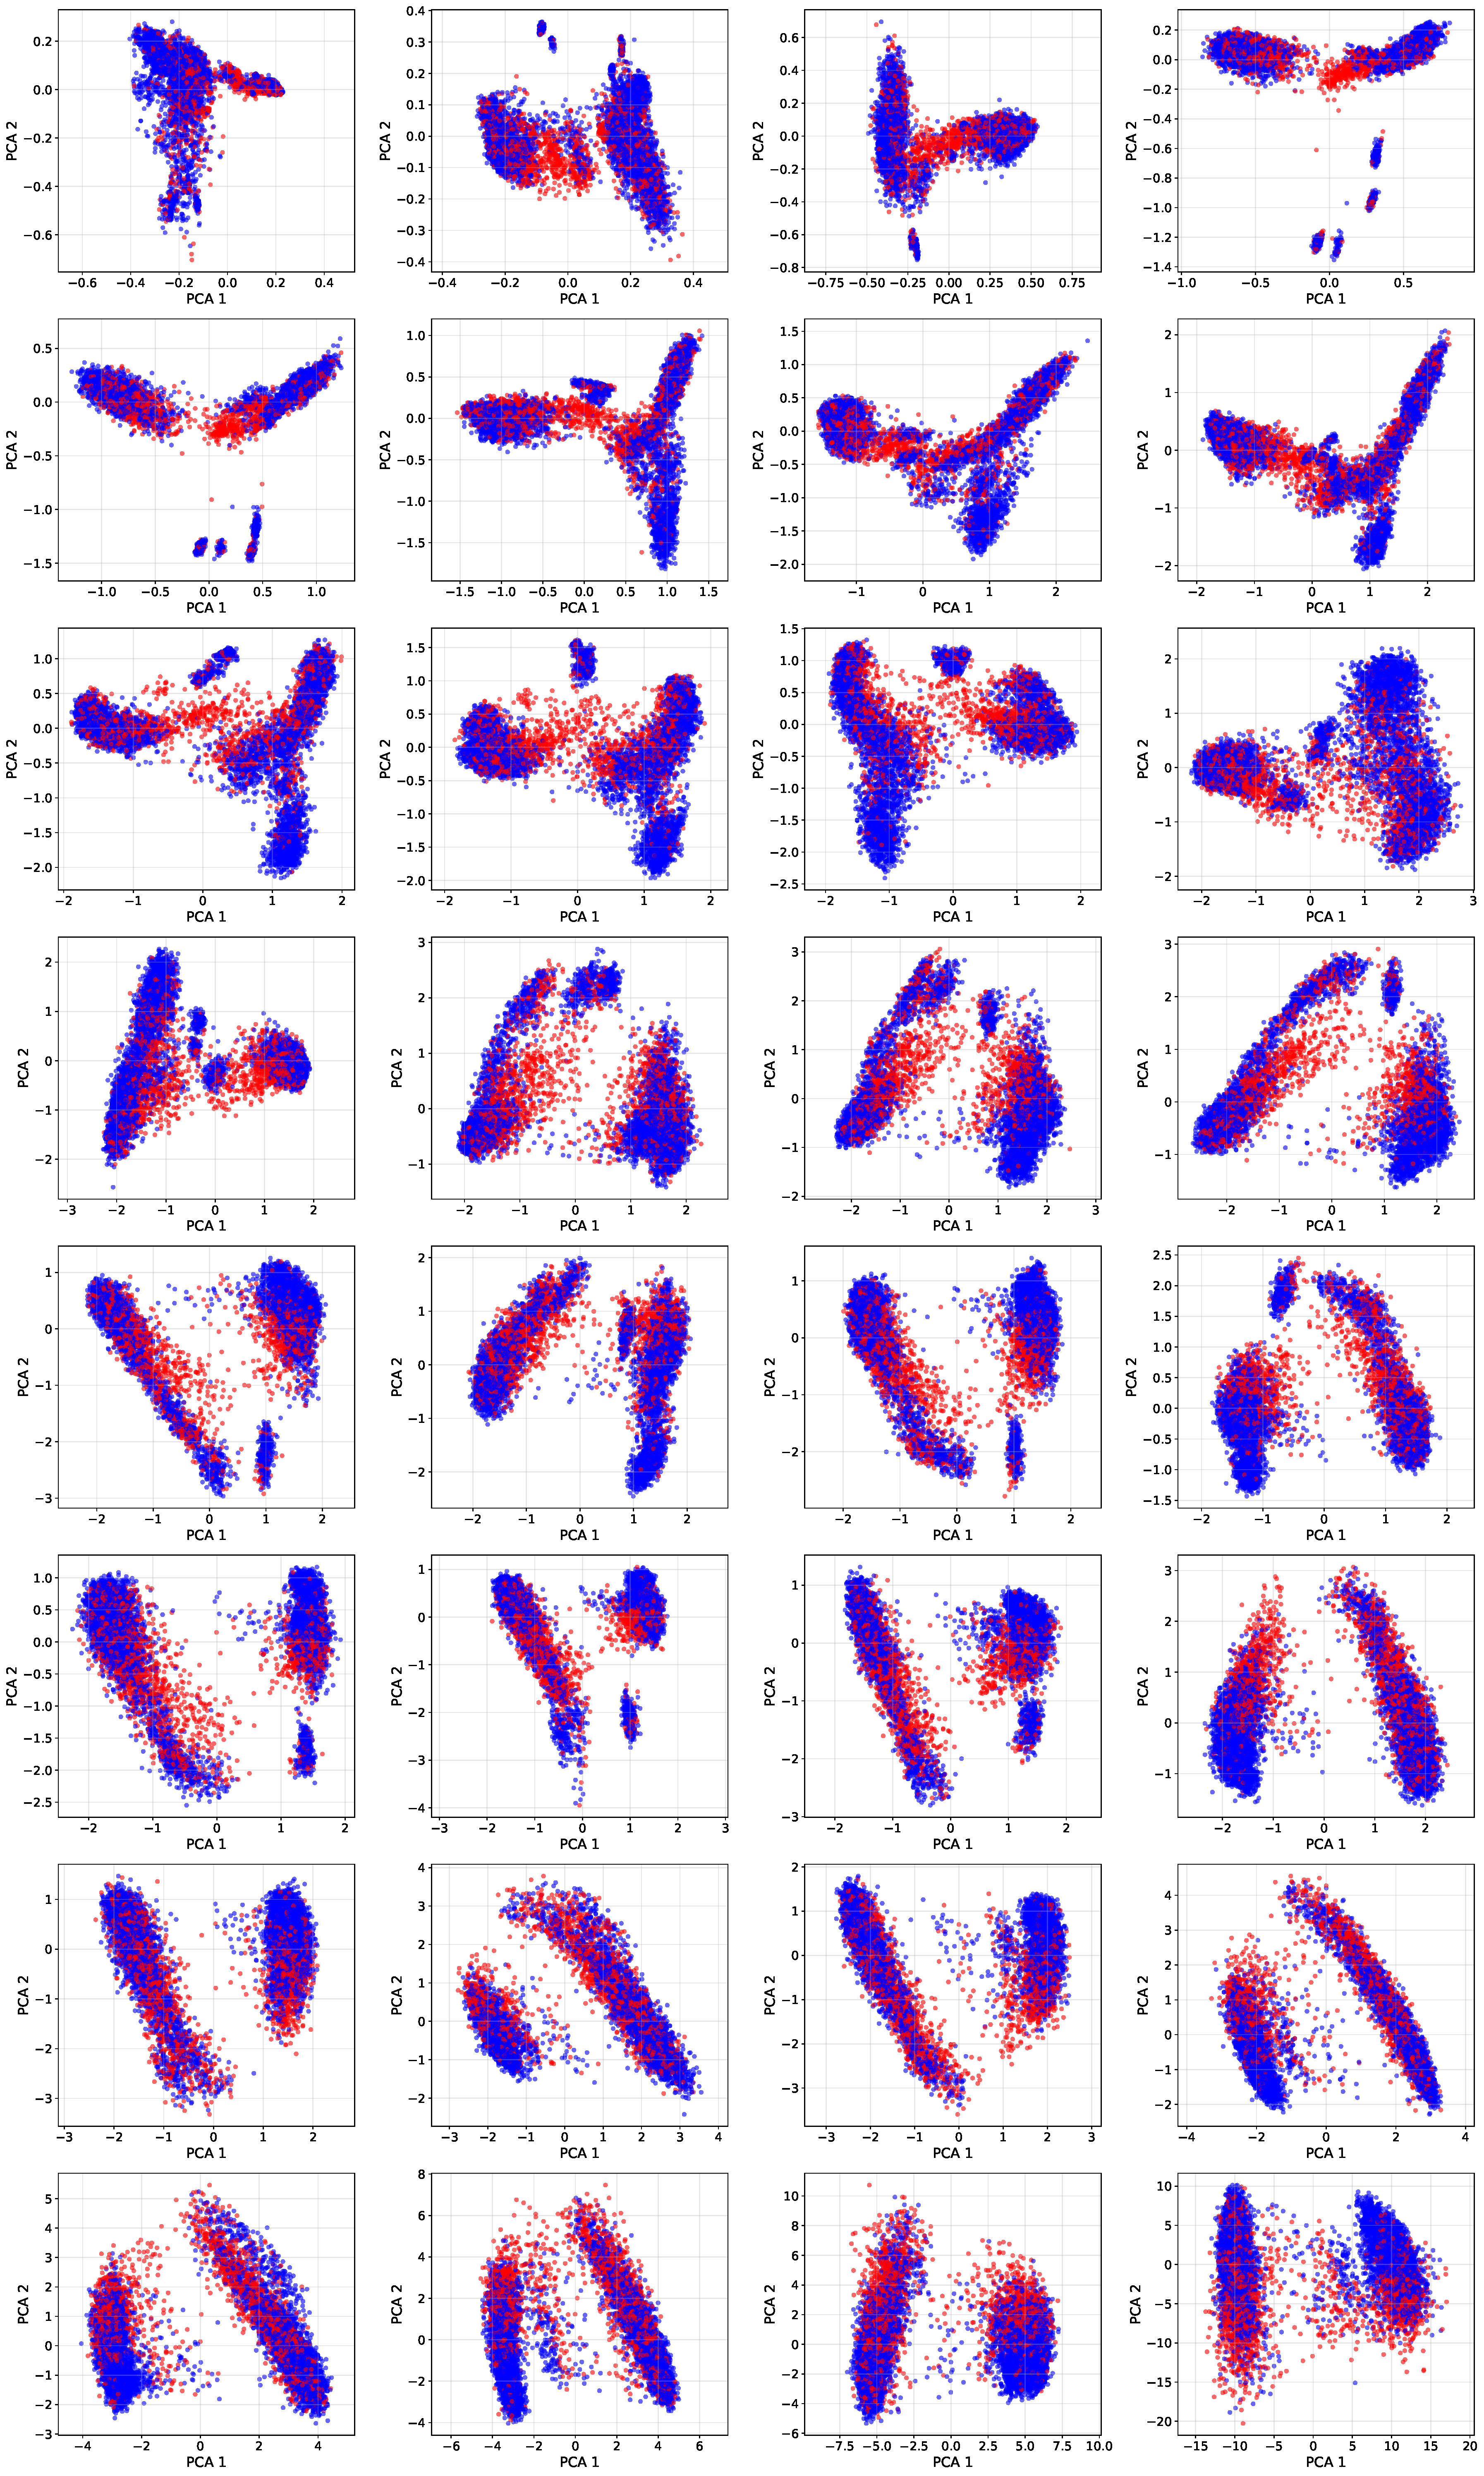
\includegraphics[width=\textwidth, height=1\textheight, keepaspectratio]{images/PCA_Plots/Llama-3.1-8B-Instruct_halu_eval_mlp_activations_PCA_CLEAN.pdf}
    \label{fig:llama-pca-mlp-he-full}
    \caption{PCA of MLP layer activations from Llama-3.1-8B-Instruct for Halu Eval}
\end{figure}



